\documentclass[10pt]{article}
\usepackage[utf8]{inputenc}
\usepackage[english]{babel}
\usepackage{amsmath}
\usepackage{graphicx}
\usepackage{float}
\usepackage{lipsum}
\usepackage{multicol}
\usepackage{xcolor}
\usepackage{tabularx}
\usepackage{booktabs}
\usepackage{array}
\usepackage{amssymb}
\usepackage{setspace}
\usepackage{subcaption}
\usepackage{microtype}
\newcolumntype{Y}{>{\centering\arraybackslash}X}
\usepackage[left=2.00cm, right=2.00cm, top=2.00cm, bottom=2.00cm]{geometry}
\setlength{\parskip}{0.3em}
\usepackage[breaklinks]{hyperref}
\usepackage{xurl}
\usepackage{caption}
\captionsetup{font=small}

% Tell LaTeX to look inside the "figures" folder for all images
\graphicspath{{figures/}}

% Code layout tool package in your preamble
\usepackage{listings}
\definecolor{mGreen}{rgb}{0,0.5,0}
\lstdefinelanguage{Dart}{
    keywords={class, const, static, int, double, bool, String, final, var, void, return, if, else, null, import, as, this, extends, factory, get, set, implements, with, operator, dynamic, show, hide, List, Uint8List, Endian, ByteData},
    keywordstyle=\color{blue}\bfseries,
    ndkeywords={@override, super},
    ndkeywordstyle=\color{darkgray}\bfseries,
    identifierstyle=\color{black},
    sensitive=true,
    comment=[l]{//},
    morecomment=[s]{/*}{*/},
    commentstyle=\color{mGreen}\itshape,
    stringstyle=\color{purple}\ttfamily,
    morestring=[b]',
    morestring=[b]"
}
\lstset{
    frame=tb,
    aboveskip=3mm,
    belowskip=3mm,
    showstringspaces=false,
    columns=flexible,
    basicstyle={\scriptsize\ttfamily},
    keywordstyle=\color{blue}\bfseries,
    commentstyle=\color{mGreen}\itshape,
    stringstyle=\color{purple},
    breaklines=true, 
    breakatwhitespace=true,  
    postbreak=\mbox{\textcolor{red}{$\hookrightarrow$}}\space,
    tabsize=2
}

\usepackage{titlesec}
\titlespacing{\section}{0pt}{12pt}{6pt}
\titlespacing{\subsection}{0pt}{6pt}{4pt}
\titleformat{\section}{\large\bfseries}{\thesection}{0.5em}{}
\titleformat{\subsection}{\normalsize\bfseries}{\thesubsection}{0.5em}{}

\begin{document}
\onehalfspacing

% =========================================================================
% TITLE PAGE
% =========================================================================
\begin{titlepage}
\centering


\includegraphics[width=0.28\textwidth]{Logo_Politecnico_Milano.png}

\vspace{0.5cm}

{\LARGE\bfseries Smart Wearables Design \& Prototyping\\[0.2cm] \par}
{\LARGE\bfseries Project Report\par}

\vspace{0.7cm}

{\Large\bfseries Group A08\par}

\vspace{0.2cm}

\begin{tabular}{c}
\normalsize Mirko Pica (274944) \\[0.17cm]
\normalsize Elena Dalle Nogare (308625) \\[0.17cm]
\normalsize Christian Prendin (286194) \\[0.17cm]
\normalsize Leonardo Grossi (280890) \\[0.17cm]
\normalsize Jaime Iriarte (295459)
\end{tabular}

\vspace{0.5cm}

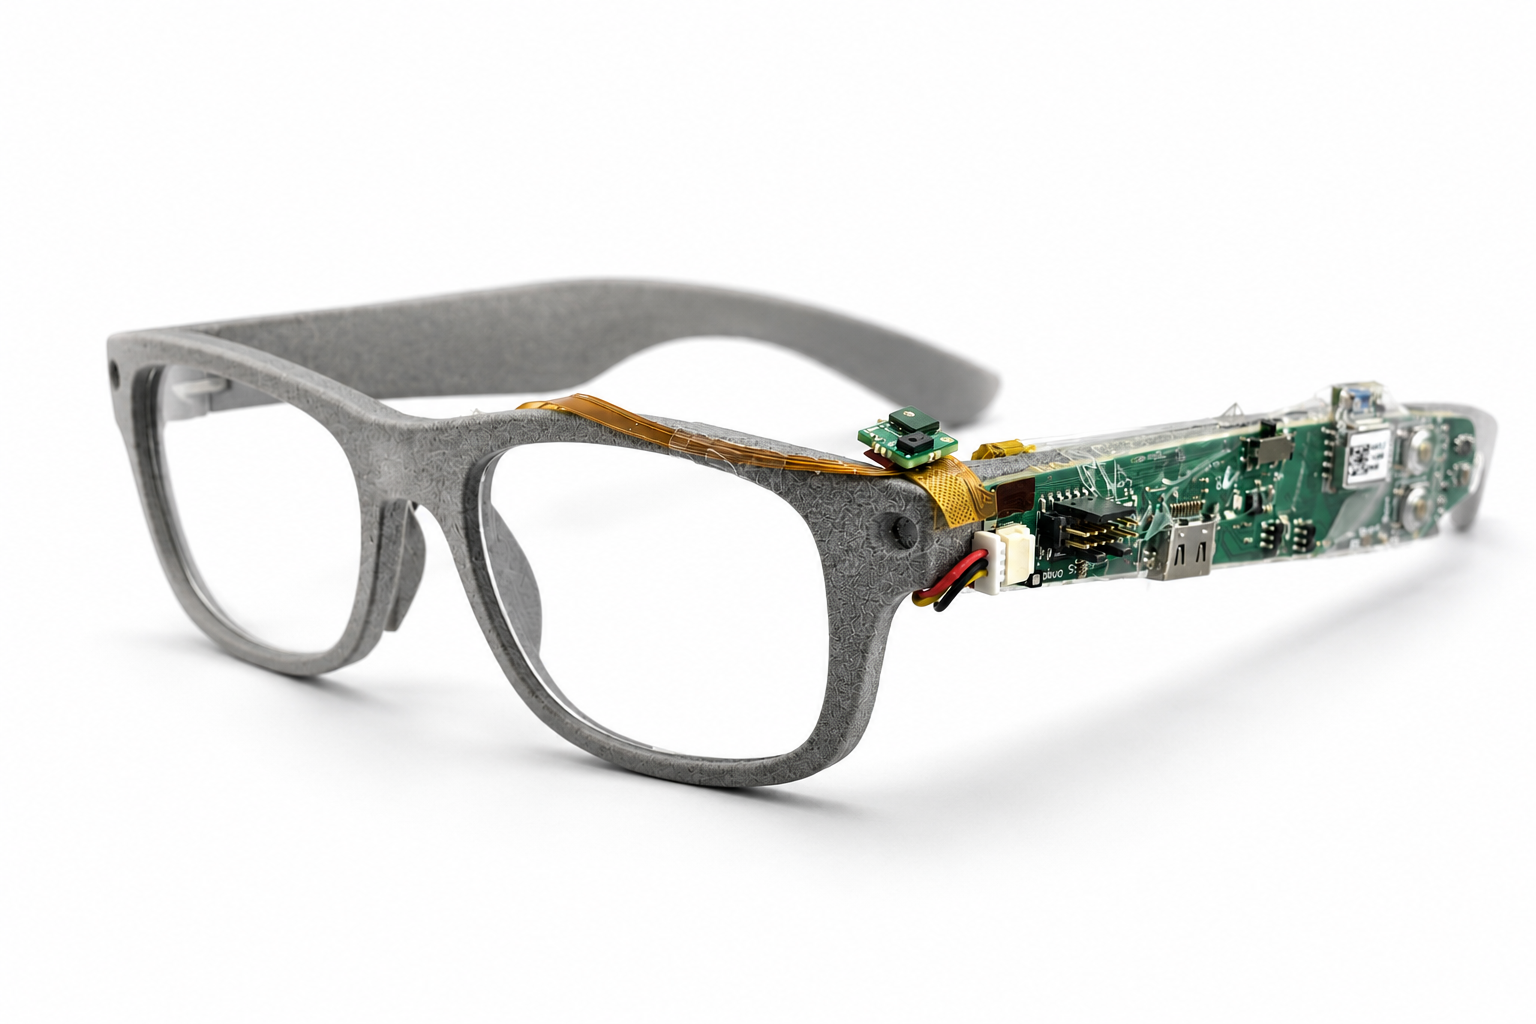
\includegraphics[width=0.9\textwidth]{Smart glasses pic.png}

\end{titlepage}

\newpage

% Start the two-column layout right from the beginning of page 2
\begin{multicols}{2}

% =========================================================================
% SECTION 1: INDIVIDUAL CONTRIBUTIONS (Max 100 words per member)
% =========================================================================
\section{Individual contributions}
\textbf{Mirko Pica:} Responsible for the embedded firmware development, focusing on the data logger state machine, the Python download utility, and the implementation of the on-device inference pipeline, while also supporting the TinyML model training phase.

\textbf{Elena Dalle Nogare:} Contributed to the hardware development of the system, with particular focus on schematic design and PCB layout implementation. Her activities included component integration, signal routing optimisation and verification of the electronic architecture of the LUMOS probe.

\textbf{Christian Prendin:} Contributed to the firmware and companion application development. His work involved the implementation of the data logger, the Bluetooth Low Energy (BLE) communication layer for inference state transmission, and the development of the Flutter smartphone application.

\textbf{Leonardo Grossi:} Worked on the development of machine learning solutions for environmental recognition through the smart glasses platform. In particular, he focused on the analysis of the data acquired from the environmental sensors, the extraction of compact audio and spectral features, the training and quantization of a lightweight context classification model, and its preparation for embedded inference on the device.

\textbf{Jaime Iriarte:} Contributed to the hardware design and implementation of the project, particularly in the development of the electronic schematics and PCB of the wearable platform. His activities included support for component integration and hardware validation procedures, while also contributing to the research and evaluation of the possible applications of the system.

Finally, all group members collaboratively contributed to the definition of the possible final applications of the project, as well as the compilation of the technical report and the demonstration video material. The system development was carried out in a parallel and coordinated manner, promoting continuous integration between hardware, firmware, and machine learning activities throughout all design, development, and validation stages.


% =========================================================================
% SECTION 2: PROJECT AIMS (Max 200 words)
% =========================================================================
\section{Project aims}
\noindent\textbf{Contributors:} Mirko Pica (20\%), Elena Dalle Nogare (20\%), Christian Prendin (20\%), Leonardo Grossi (20\%), Jaime Iriarte (20\%)
\vspace{0.1cm}

The primary aim of this project is to develop an autonomous, context-aware smart glasses platform that processes environmental data locally at the edge. The system is engineered to eliminate cloud dependency by executing real-time machine learning inference directly on an embedded microcontroller.

To achieve this, the project focuses on three core development objectives:
\begin{enumerate}
    \item \textbf{Hardware Expansion:} Designing and manufacturing the custom 4-layer LUMOS probe PCB to integrate an AS7341 multispectral light sensor ($I^2C$) and an IMP34DT05TR digital MEMS microphone (PDM).
    \item \textbf{On-Chip TinyML Engine:} Training and deploying a compressed, 8-bit quantized Artificial Neural Network (ANN) onto an STM32U575 MCU to classify five environmental contexts (Underground, Outdoor, Indoor Quiet, Indoor Normal, Covered/Dark) from a set of features extracted from multispectral light measurements and audio signals and computed on-device.
    \item \textbf{Wireless Synchronization:} Implementing a firmware state machine that transmits classified state flags via Bluetooth Low Energy (BLE) to trigger dynamic, context-aware UI features in a companion smartphone application.
\end{enumerate}

The complete open-source firmware, hardware design files, and mobile application source code are publicly hosted on GitHub at \url{https://github.com/M1RK02/LumiaGlasses}.

% =========================================================================
% SECTION 3: HARDWARE DESIGN (Max 500 words + Figures)
% =========================================================================
\section{Hardware design}
\noindent\textbf{Contributors:} Elena Dalle Nogare (50\%), Jaime Iriarte (50\%)
\vspace{0.1cm}

The hardware architecture of the smart glasses is based on a modular wearable electronics platform composed of a main board, a flexible interconnection board, and a custom-designed sensor probe. While the main board and interconnection flex were provided as a pre-existing base platform, our hardware design work focused exclusively on the schematic capture, layout, routing, and fabrication of the custom LUMOS sensor probe PCB. The main board is designed around the STM32U575 ultra-low-power microcontroller, selected for its reduced power consumption, integrated peripherals, and suitability for embedded edge-computing applications.

The main board integrates the STM32U575 MCU, NAND flash memory for local data logging, USB communication, battery management circuitry, and a BLE communication module (RN4871). The board also includes the LSM6DSO16IS inertial measurement unit, which was not utilized in the scope of this environmental context-recognition project. Wireless communication through BLE enables real-time transmission of classified context tags to the companion mobile application.

The custom LUMOS probe integrates two environmental sensors: the AS7341 multispectral light sensor and the IMP34DT05TR digital MEMS microphone. The AS7341 sensor enables acquisition of ambient light information across multiple wavelength bands, while the MEMS microphone provides low-power audio acquisition through a PDM interface. Both sensors were selected because of their compact dimensions and low-power operation, making them suitable for wearable applications. The resulting probe PCB is shown in Figures~\ref{fig:lumos_top} and~\ref{fig:lumos_bottom}. 

The electrical schematics of the probe are reported in Figures~\ref{fig:light_sensor_schematic}, \ref{fig:microphone_schematic}, and \ref{fig:connector_schematic}. The AS7341 multispectral sensor was interfaced through the I2C bus operating at 1.8~V with dedicated pull-up resistors, while the IMP34DT05TR microphone was connected through a PDM interface using dedicated clock and data lines. The probe was connected to the main board through a compact board-to-board connector optimized for wearable integration.

The custom LUMOS probe hardware was implemented on a four-layer PCB stack-up using Altium Designer to improve signal integrity and power distribution. The probe stack-up consists of a top signal layer dedicated to sensors and routing, an internal ground plane, an internal power plane, and a bottom signal layer used for the probe connector and additional routing. Dedicated ground planes and local decoupling capacitors were used on the probe to reduce noise and improve the stability of both the analog and digital domains. The probe PCB routing was optimized to minimize board dimensions while maintaining accessibility for debugging and testing. Communication between peripherals and the microcontroller was implemented using multiple interfaces according to the sensor requirements. In particular, the multispectral sensor communicates through I2C, while the NAND memory uses SPI communication. The digital microphone was interfaced through a PDM audio connection.

To assess commercial viability, a production cost analysis was conducted for a small manufacturing batch of 125 units. The total estimated production cost per LUMOS probe is €8.8, broken down in Table~\ref{tab:bom_cost}.

\begin{table}[H]
\centering

\label{tab:bom_cost}
\resizebox{\columnwidth}{!}{%
\begin{tabular}{llcc}
\toprule
\textbf{Component / Service} & \textbf{Description} & \textbf{Cost (\text{€})} \\
\midrule
AS7341 & Multispectral Spectral Sensor & 5.21 \\
IMP34DT05TR & Digital MEMS Microphone         & 1.81 \\
DF40C-10DP-0.4V & 10-pin Board-to-Board Conn.   & 0.59 \\
0402YC104JAT4A & Ceramic Capacitor 0.1uF      & 0.02 \\
0402YD105KAT4A & Ceramic Capacitor 1uF      & 0.10 \\
CR0201-JW-472GLF & Fixed resistor 4.7 k$\Omega$      & 0.01 \\
PCB Fabrication & 4-Layer FR4 (JLC\text{PCB})      & 0.35 \\
PCBA Assembly & Automated SMT Placement           & 0.71 \\
\midrule
\textbf{Total Cost} & \textbf{Per Unit Production Base} & \textbf{\text{€}8.8} \\
\bottomrule
\end{tabular}%
}
\caption{Bill of Materials (BOM) and production cost breakdown per unit for a 125-unit manufacturing run of the LUMOS probe.}
\label{tab:bom_cost}
\end{table}

% =========================================================================
% SECTION 4: FIRMWARE AND SOFTWARE DEVELOPMENT (Max 500 words + Code)
% =========================================================================
\section{Firmware development}
\noindent\textbf{Contributors:} Mirko Pica (60\%), Christian Prendin (10\%), Leonardo Grossi (30\%)
\vspace{0.1cm}

The software ecosystem for the context-aware smart glasses is split into an embedded dual-firmware pipeline (on-chip logging and inference) and a python data processing framework.

\subsection{Data Logger Firmware Architecture}
The data collection firmware operates as an event-driven Finite State Machine on the STM32U575 MCU. Multispectral data from the AS7341 are acquired non-blocking over I2C3 by utilizing the sensor's physical interrupt pin to signal when new spectral integrations are complete, while the digital microphone feeds PDM data directly to the Multi-Function Digital Filter (MDF1) block. To guarantee zero data loss at a 16~kHz audio sampling rate, a circular GPDMA1 double-buffering scheme is implemented using a partitioned array (\texttt{AUDIO\_BLOCK\_SIZE} = 2034). Half-transfer and full-transfer interrupts handle time-stamping, data packet structuring, and local flash logging synchronously.

\subsection{Python Script: Data Retrieval \& Processing}
An offline Python utility handles data retrieval via USB Virtual COM Port (VCP). It communicates with the MCU state machine in download mode, parsing the raw data packets streamed from the NAND memory into organized structural arrays (Time, Light Channels, Raw Audio).

\subsection{Python Script: TinyML Model Training}
The training notebook extracts spectral descriptors and time-domain acoustic audio parameters. A lightweight Artificial Neural Network (ANN) model is built in TensorFlow/Keras to perform 5-class context classification. The pipeline applies post-training 8-bit integer quantization, exporting an optimized \texttt{.tflite} flatbuffer. We subsequently used the STM32Cube.AI (X-CUBE-AI) expansion pack to convert the TFLite flatbuffer model into optimized C code for embedded microcontroller execution.

\subsection{TinyML Model and Quantization}
The on-device classifier is a Multilayer Perceptron (MLP) neural network trained to classify the five environmental contexts. The network processes a 39-dimensional feature set containing light intensity, spectral ratios, darkness level, flicker frequency distribution, audio energy, silence ratio, zero-crossing rate, and frequency-band energy. The architecture consists of 39 input features, two hidden layers (32 and 16 neurons with ReLU activation), and a 5-class Softmax output layer. The model was optimized using post-training 8-bit integer quantization (INT8) and converted to C code via STM32Cube.AI for deployment on the STM32U575 microcontroller.

\subsection{Embedded Inference Firmware Deployment}
The deployment firmware drops logging tasks, integrates the TinyML runtime engine, and implements low-power optimizations. To maximize battery life, the firmware was refactored to decouple high-priority hardware data ingestion from execution. Lightweight interrupt handlers (GPDMA and EXTI) only buffer incoming data and set atomic trigger flags, dispatching heavy feature extraction and network evaluation to the main thread. When idle, the CPU transitions into a low-power Wait-For-Interrupt (WFI) state via \texttt{HAL\_PWR\_EnterSLEEPMode()}, gating the core clock while peripherals continue autonomous DMA data collection in SRAM. A critical section using global interrupt masking is implemented during the state checks to prevent sleep-race conditions (lost wakeups).

\subsection{Core Processing Implementation Code}
The primary implementation algorithms spanning embedded acquisition, data retrieval, network compilation, edge inference, and application decoding are presented below:

\begin{lstlisting}[language=C, caption=Embedded Data Logger MDF DMA Capture Callbacks]
// DMA Half-Complete Callback for Initial Buffer Block
void HAL_MDF_AcqHalfCpltCallback(MDF_HandleTypeDef *hmdf) {
  if (hmdf->Instance == MDF1_Filter0 && current_state == STATE_ACQUISITION) {
    write_packet(NAND_packet, packet_index, spectral_data_ready, &spectral_data_buffer, &audio_circular_buffer[0]);
    spectral_data_ready = false;
    packet_index++; sample++; write_memory();
  }
}

// DMA Complete Callback for Secondary Buffer Block
void HAL_MDF_AcqCpltCallback(MDF_HandleTypeDef *hmdf) {
  if (hmdf->Instance == MDF1_Filter0 && current_state == STATE_ACQUISITION) {
    write_packet(NAND_packet, packet_index, spectral_data_ready, &spectral_data_buffer, &audio_circular_buffer[BLOCK_AUDIO_SAMPLES]);
    spectral_data_ready = false;
    packet_index++; sample++; write_memory();
  }
}
\end{lstlisting}

\begin{lstlisting}[language=Python, caption=Python Script for VCP Memory Download]
import serial, struct
def receive_and_save_data(ser, bin_filename, packet_size=4096):
  with open(bin_filename, "wb") as f:
    while True:
      data = ser.read(packet_size)
      if not data: continue
      if data == b"T": break # Terminator character
      f.write(data)

# Packet format for processing binary log files
packet_dtype = np.dtype([
  ("start_char", "S1"),       # 1 byte ('S')
  ("packet_index", "<u2"),    # 2 bytes
  ("spectral_flag", "u1"),    # 1 byte
  ("f1", "<u2"), ("f2", "<u2"), ("f3", "<u2"), ("f4", "<u2"),
  ("f5", "<u2"), ("f6", "<u2"), ("f7", "<u2"), ("f8", "<u2"),
  ("clear", "<u2"), ("nir", "<u2"),
  ("flickering_type", "<u4"), # 4 bytes
  ("audio", "<i2", 2034),     # 4068 bytes audio block (2034 int16)
])
\end{lstlisting}

\begin{lstlisting}[language=Python, caption=TensorFlow Optimization and TFLite Export]
import tensorflow as tf
# Perform post-training integer-only quantization
converter = tf.lite.TFLiteConverter.from_keras_model(model)
converter.optimizations = [tf.lite.Optimize.DEFAULT]
converter.representative_dataset = representative_dataset
converter.target_spec.supported_ops = [tf.lite.OpsSet.TFLITE_BUILTINS_INT8]
converter.inference_input_type = tf.int8
converter.inference_output_type = tf.int8
tflite_quant_model = converter.convert()
\end{lstlisting}

\begin{lstlisting}[language=C, caption=On-Chip TinyML Inference Loop Execution]
// ISR Context (Lightweight logging & flag dispatch)
void Ingest_Block_To_Sliding_Window(int16_t* raw_audio_source) {
  memcpy(audio_window_history[write_ptr], raw_audio_source, BLOCK_AUDIO_SAMPLES * sizeof(int16_t));
  write_ptr = (write_ptr + 1) % WINDOW_PACKET_COUNT;
  if (blocks_accumulated == WINDOW_PACKET_COUNT && stride_counter >= INFERENCE_STRIDE_PACKETS) {
    stride_counter = 0;
    processing_write_ptr = write_ptr;
    data_processing_requested = 1; // Dispatch to main thread context
  }
}

// Thread Context (Main Loop Dispatcher)
while (1) {
  if (data_processing_requested) {
    data_processing_requested = 0;
    Reconstruct_Audio_Scratchpad(processing_write_ptr);
    Extract_Spectro_Features_Window(spectro_window_history, nn_input_features_float);
    Extract_Flicker_Features_Window(flicker_window_history, WINDOW_PACKET_COUNT, nn_input_features_float);
    Extract_Audio_Features_Window(audio_processing_scratchpad, TOTAL_WINDOW_SAMPLES, nn_input_features_float);
    Apply_Normalization(nn_input_features_float);
    
    for (int i = 0; i < AI_NETWORK_IN_1_SIZE; i++) {
      float q_val = roundf(nn_input_features_float[i] / 0.0541030541062355f) - 71.0f;
      nn_input_features[i] = (int8_t)__SSAT((int32_t)q_val, 8);
    }
    
    ai_network_run(network_instance, &ai_input[0], &ai_output[0]);
    uint8_t winning_class_idx = Get_Max_Probability(nn_output_predictions);
    BLE_SendLumosPacket(winning_class_idx, &spectral_data_buffer); // Transmit context
  }

  // Safe atomic Wait-For-Interrupt low-power entry
  __disable_irq();
  if (!data_processing_requested) {
    HAL_PWR_EnterSLEEPMode(PWR_MAINREGULATOR_ON, PWR_SLEEPENTRY_WFI);
  }
  __enable_irq();
}
\end{lstlisting}

\begin{lstlisting}[language=Dart, caption=Flutter Dart Companion App BLE Packet Parser]
class PacketParser {
  static const int packetLength = 24;
  static const int _startByte  = 0x7B; // '{'
  static const int _typeByte   = 0x4C; // 'L'
  static const int _endByte    = 0x7D; // '}'

  static LumosPacket? parse(List<int> raw) {
    if (raw.length != packetLength || raw[0] != _startByte || raw[1] != _typeByte || raw[23] != _endByte) return null;

    final bd = Uint8List.fromList(raw.sublist(2, 23)).buffer.asByteData();
    return LumosPacket(
      classLabel: bd.getUint8(0),
      f1: bd.getUint16(1, Endian.little),
      f2: bd.getUint16(3, Endian.little),
      clear: bd.getUint16(17, Endian.little),
      nir:   bd.getUint16(19, Endian.little),
    );
  }
}
\end{lstlisting}

% =========================================================================
% SECTION 5: OPTIONAL IMPROVEMENTS (Max 250 words + Figures)
% =========================================================================
\section{Optional improvements}
\noindent\textbf{Contributors:} Leonardo Grossi (20\%), Christian Prendin (80\%)
\vspace{0.1cm}

To enhance the smart glasses platform with consumer-oriented functionalities, a companion mobile application was developed using Flutter. 

The application establishes a BLE connection with the smart glasses, receiving the environmental classification packets in real time. Instead of streaming raw telemetry, the application decodes the 24-byte packet to retrieve the current environment class and spectral light levels. A local state management provider updates the mobile user interface dynamically based on the detected environment (e.g., triggering quiet UI states, dark theme transitions, or displaying real-time spectral channel charts as shown in Figure~\ref{fig:mobile_app_screens}).

\begin{figure}[H]
    \centering
    \begin{subfigure}[t]{0.25\linewidth}
        \centering
        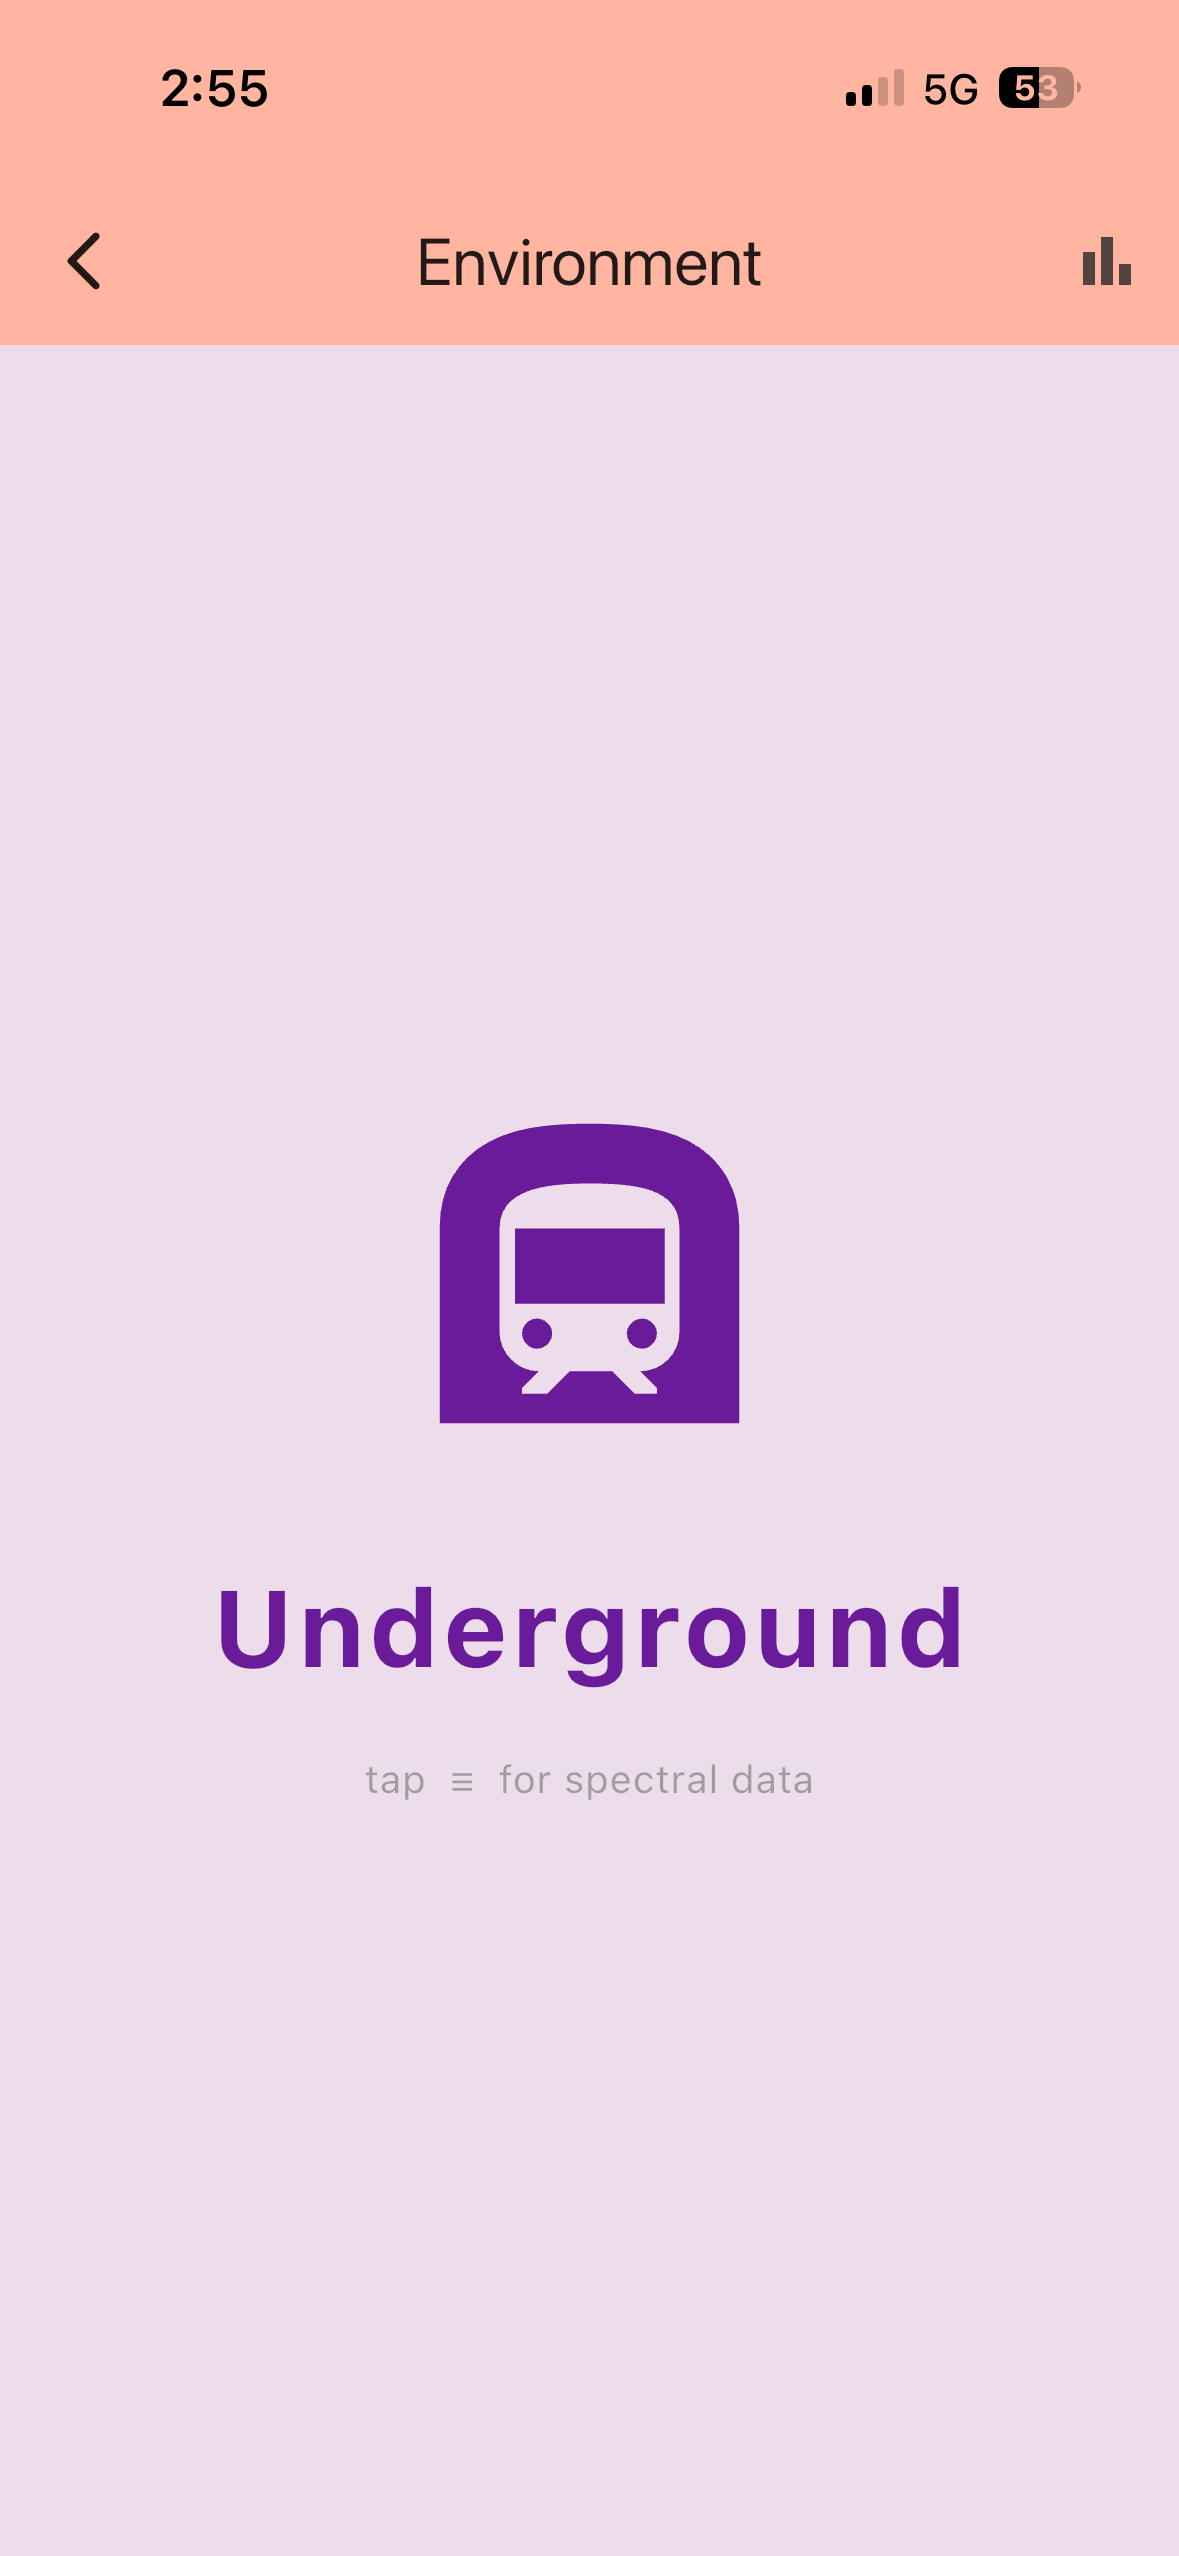
\includegraphics[width=\linewidth]{app_underground.PNG}
        \caption{Underground}
        \label{fig:app_underground}
    \end{subfigure}
    \hfill
    \begin{subfigure}[t]{0.25\linewidth}
        \centering
        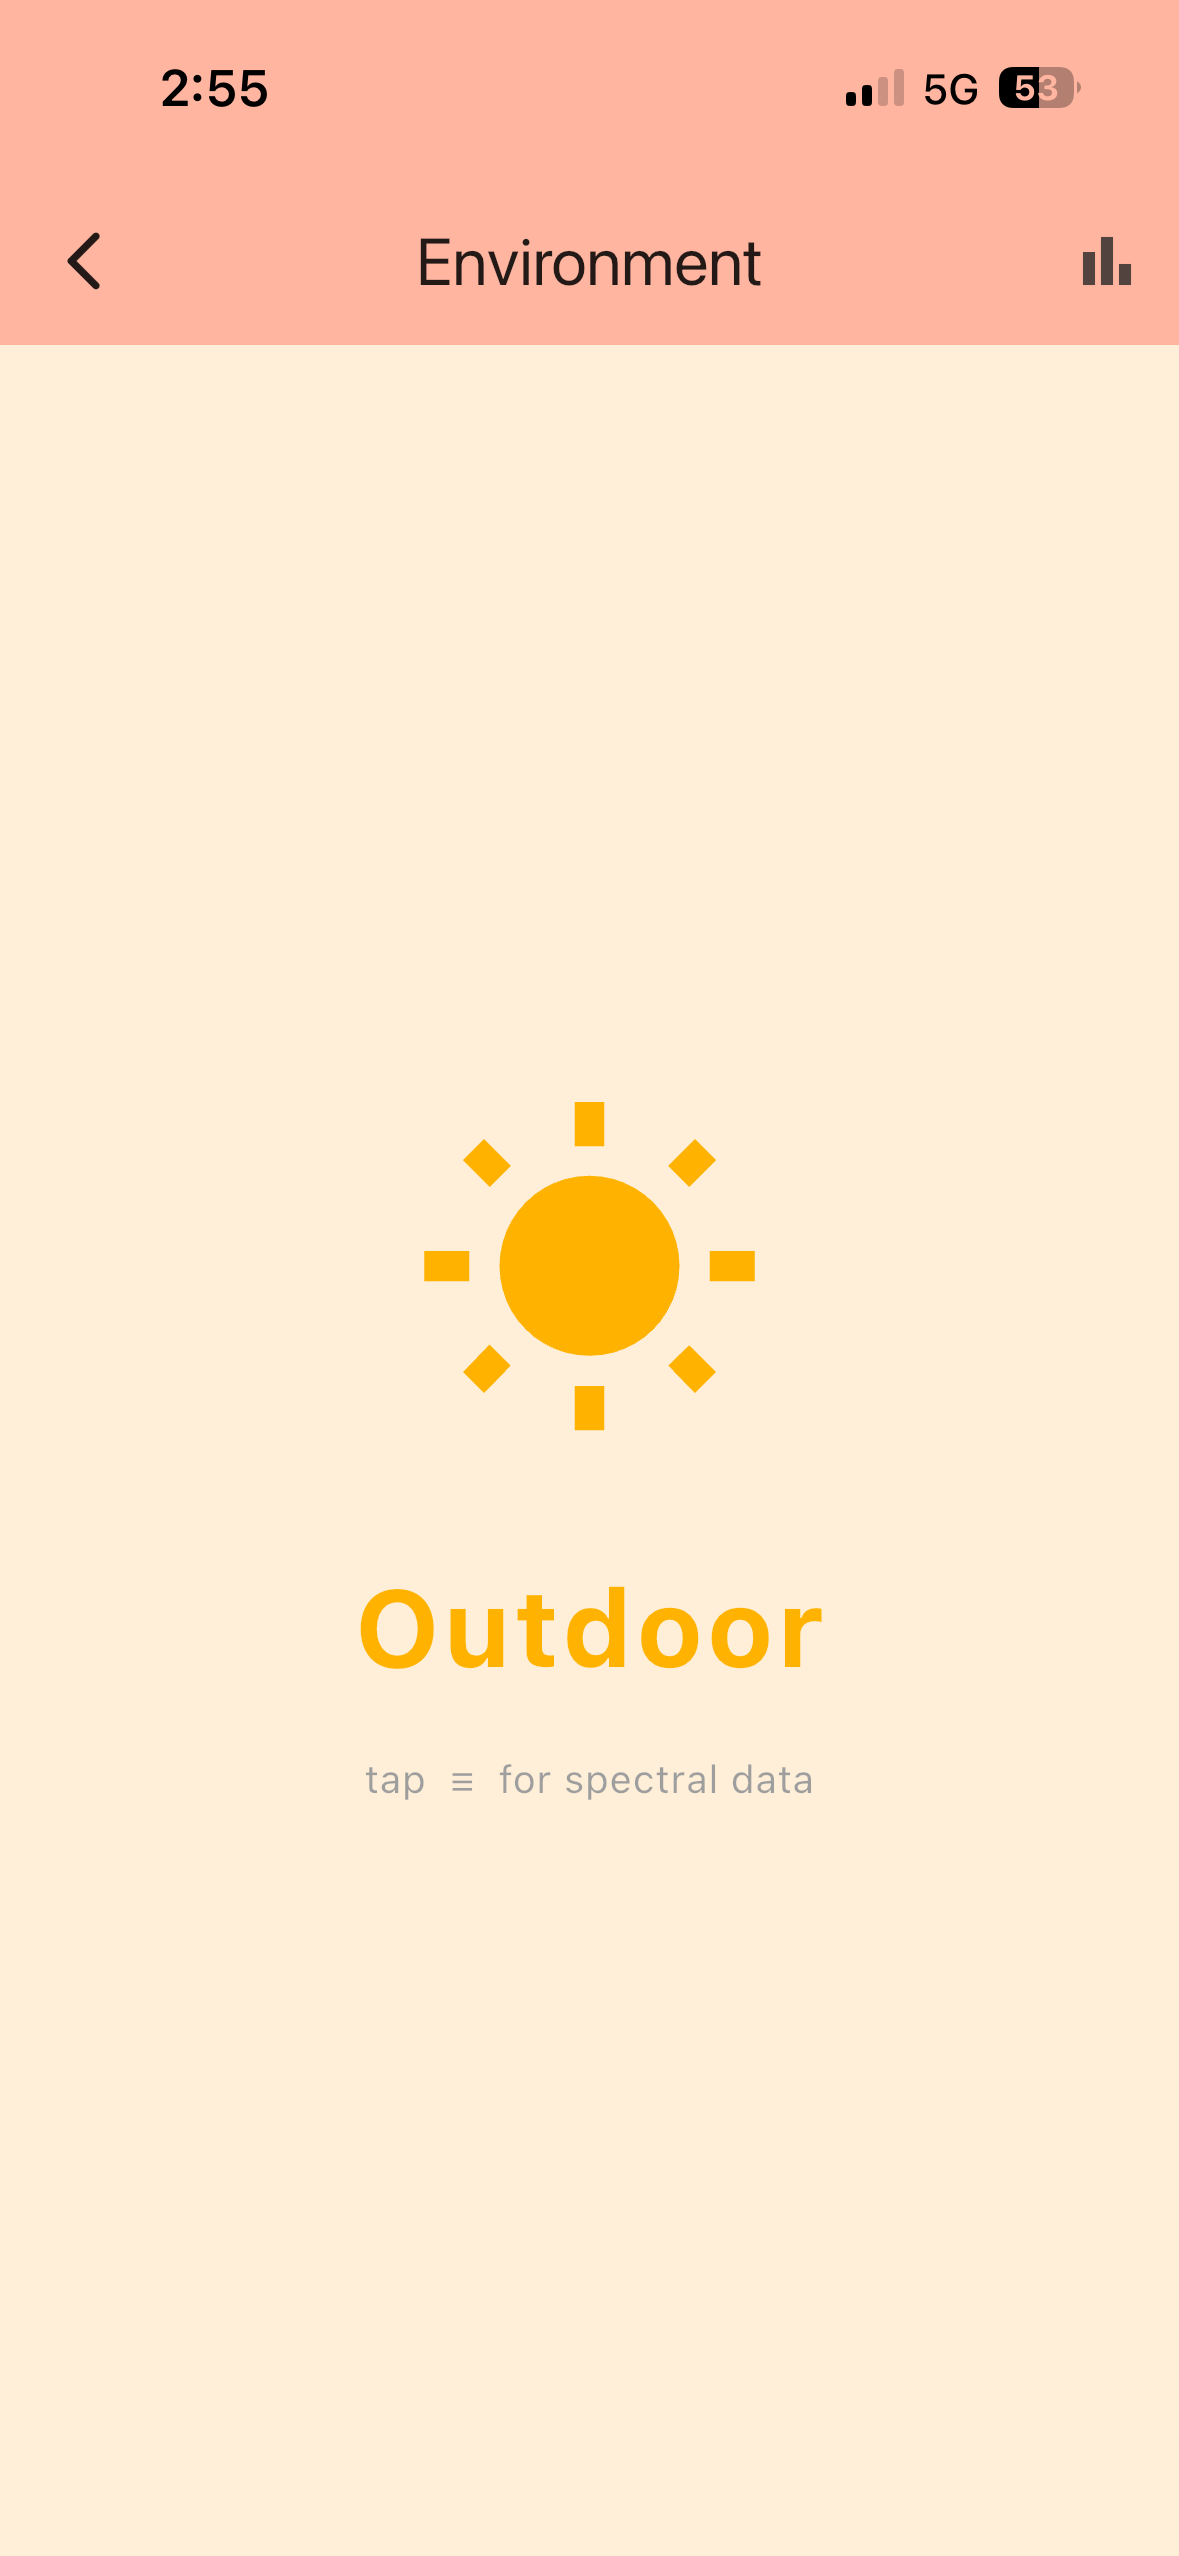
\includegraphics[width=\linewidth]{app_outdoor.PNG}
        \caption{Outdoor}
        \label{fig:app_outdoor}
    \end{subfigure}
    \hfill
    \begin{subfigure}[t]{0.25\linewidth}
        \centering
        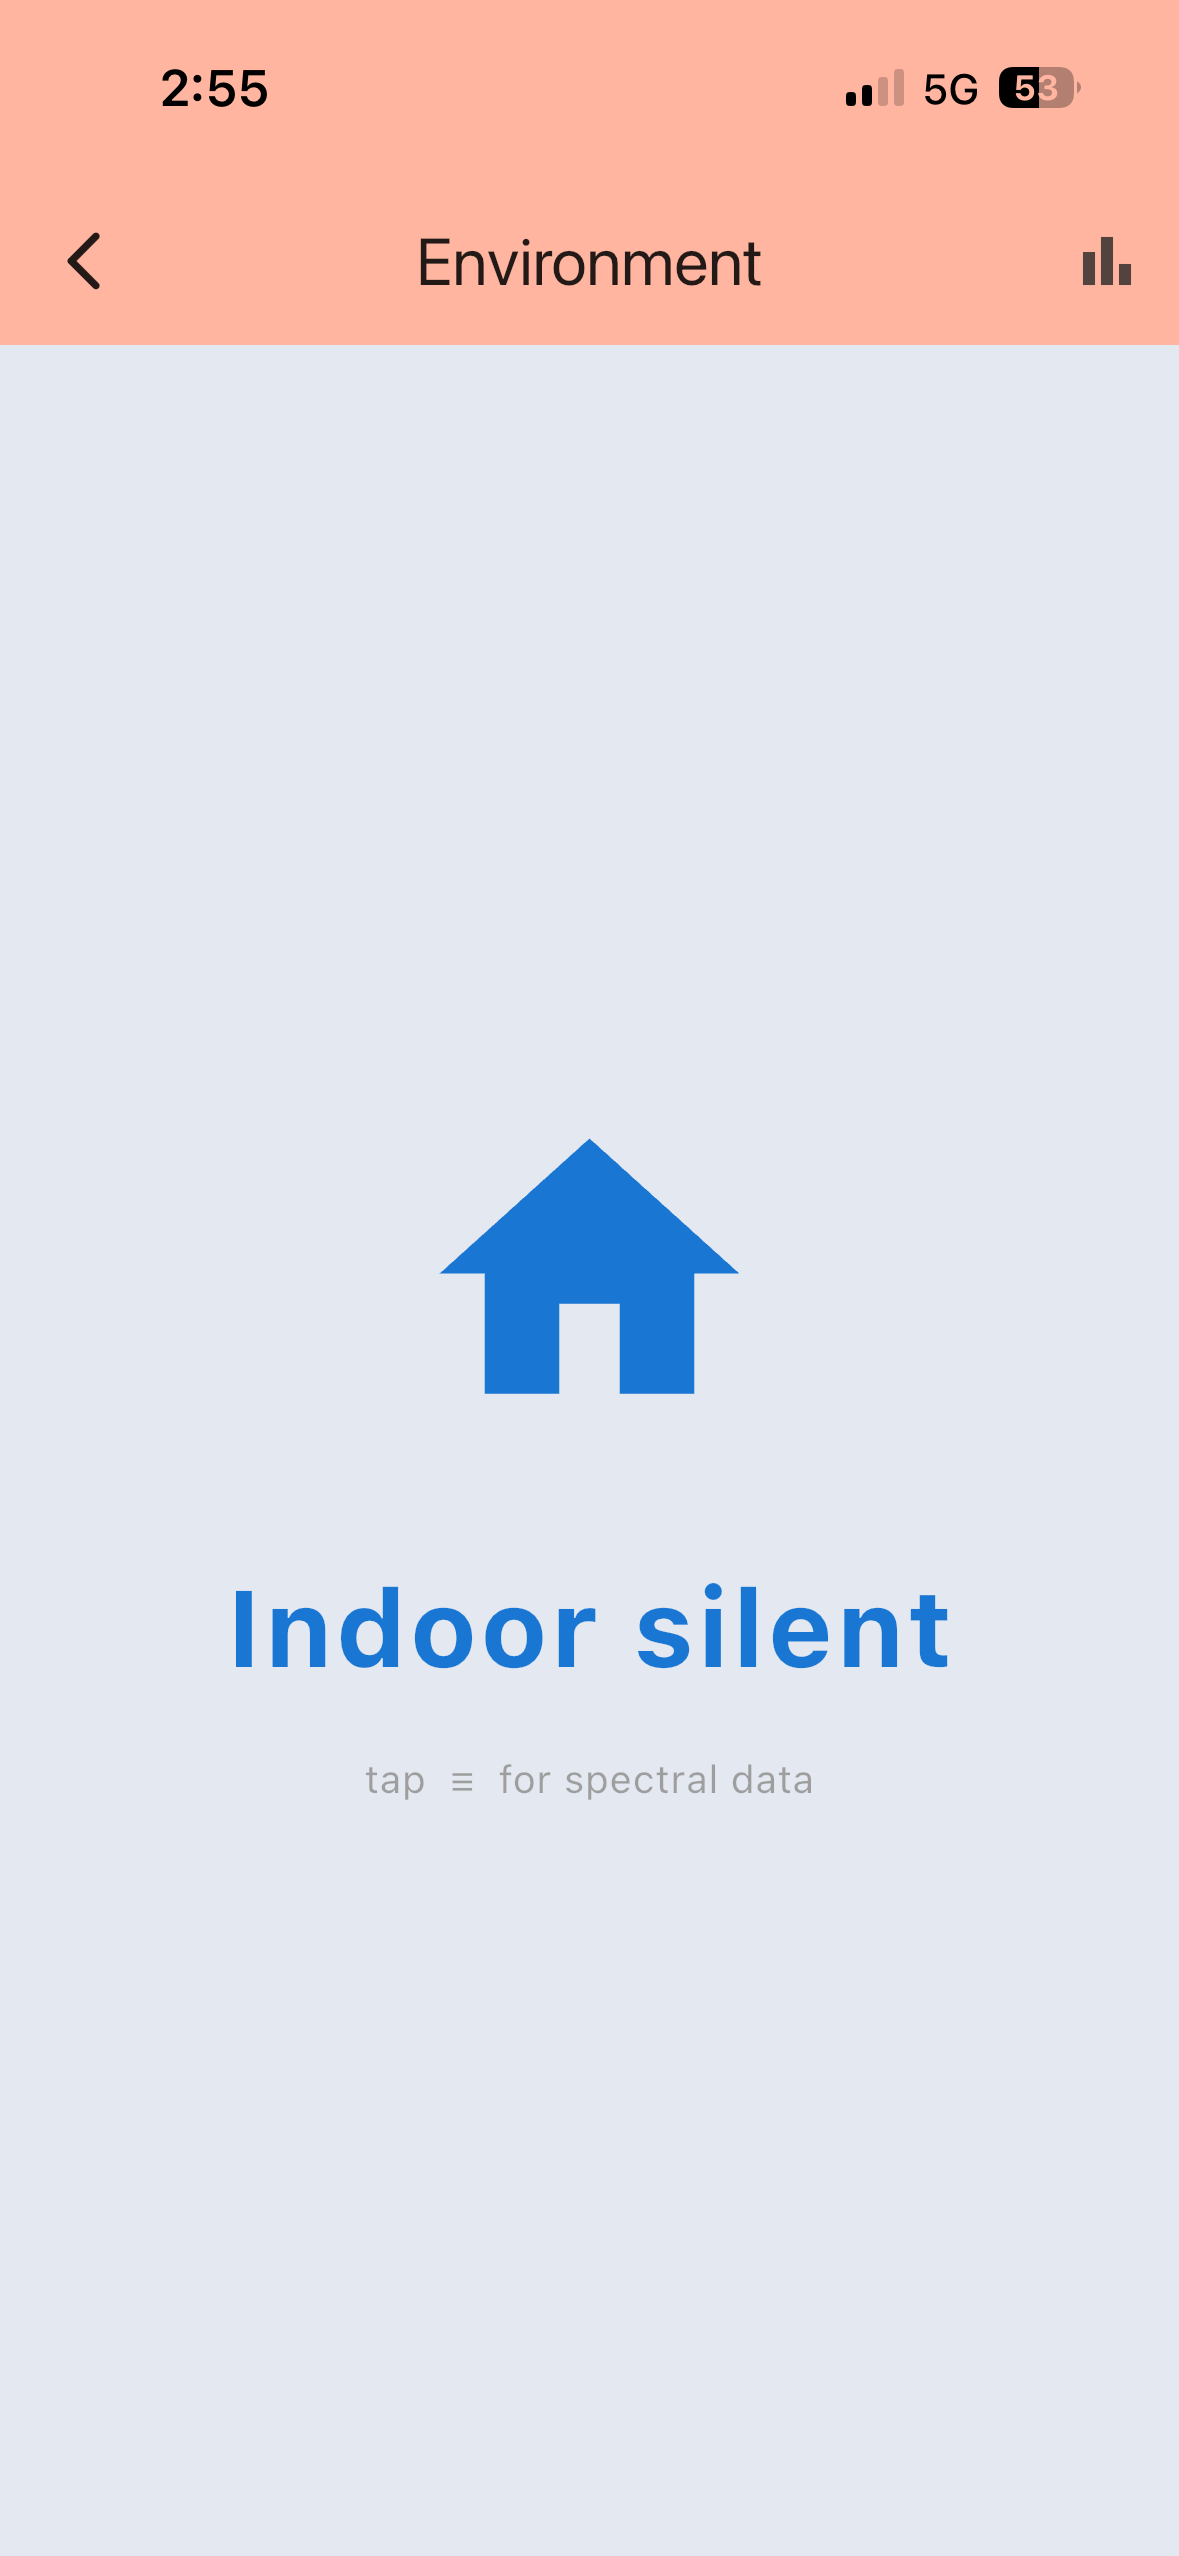
\includegraphics[width=\linewidth]{app_indoor_silent.PNG}
        \caption{Indoor Silent}
        \label{fig:app_indoor_silent}
    \end{subfigure}
    
    \vspace{0.2cm}
    
    \begin{subfigure}[t]{0.25\linewidth}
        \centering
        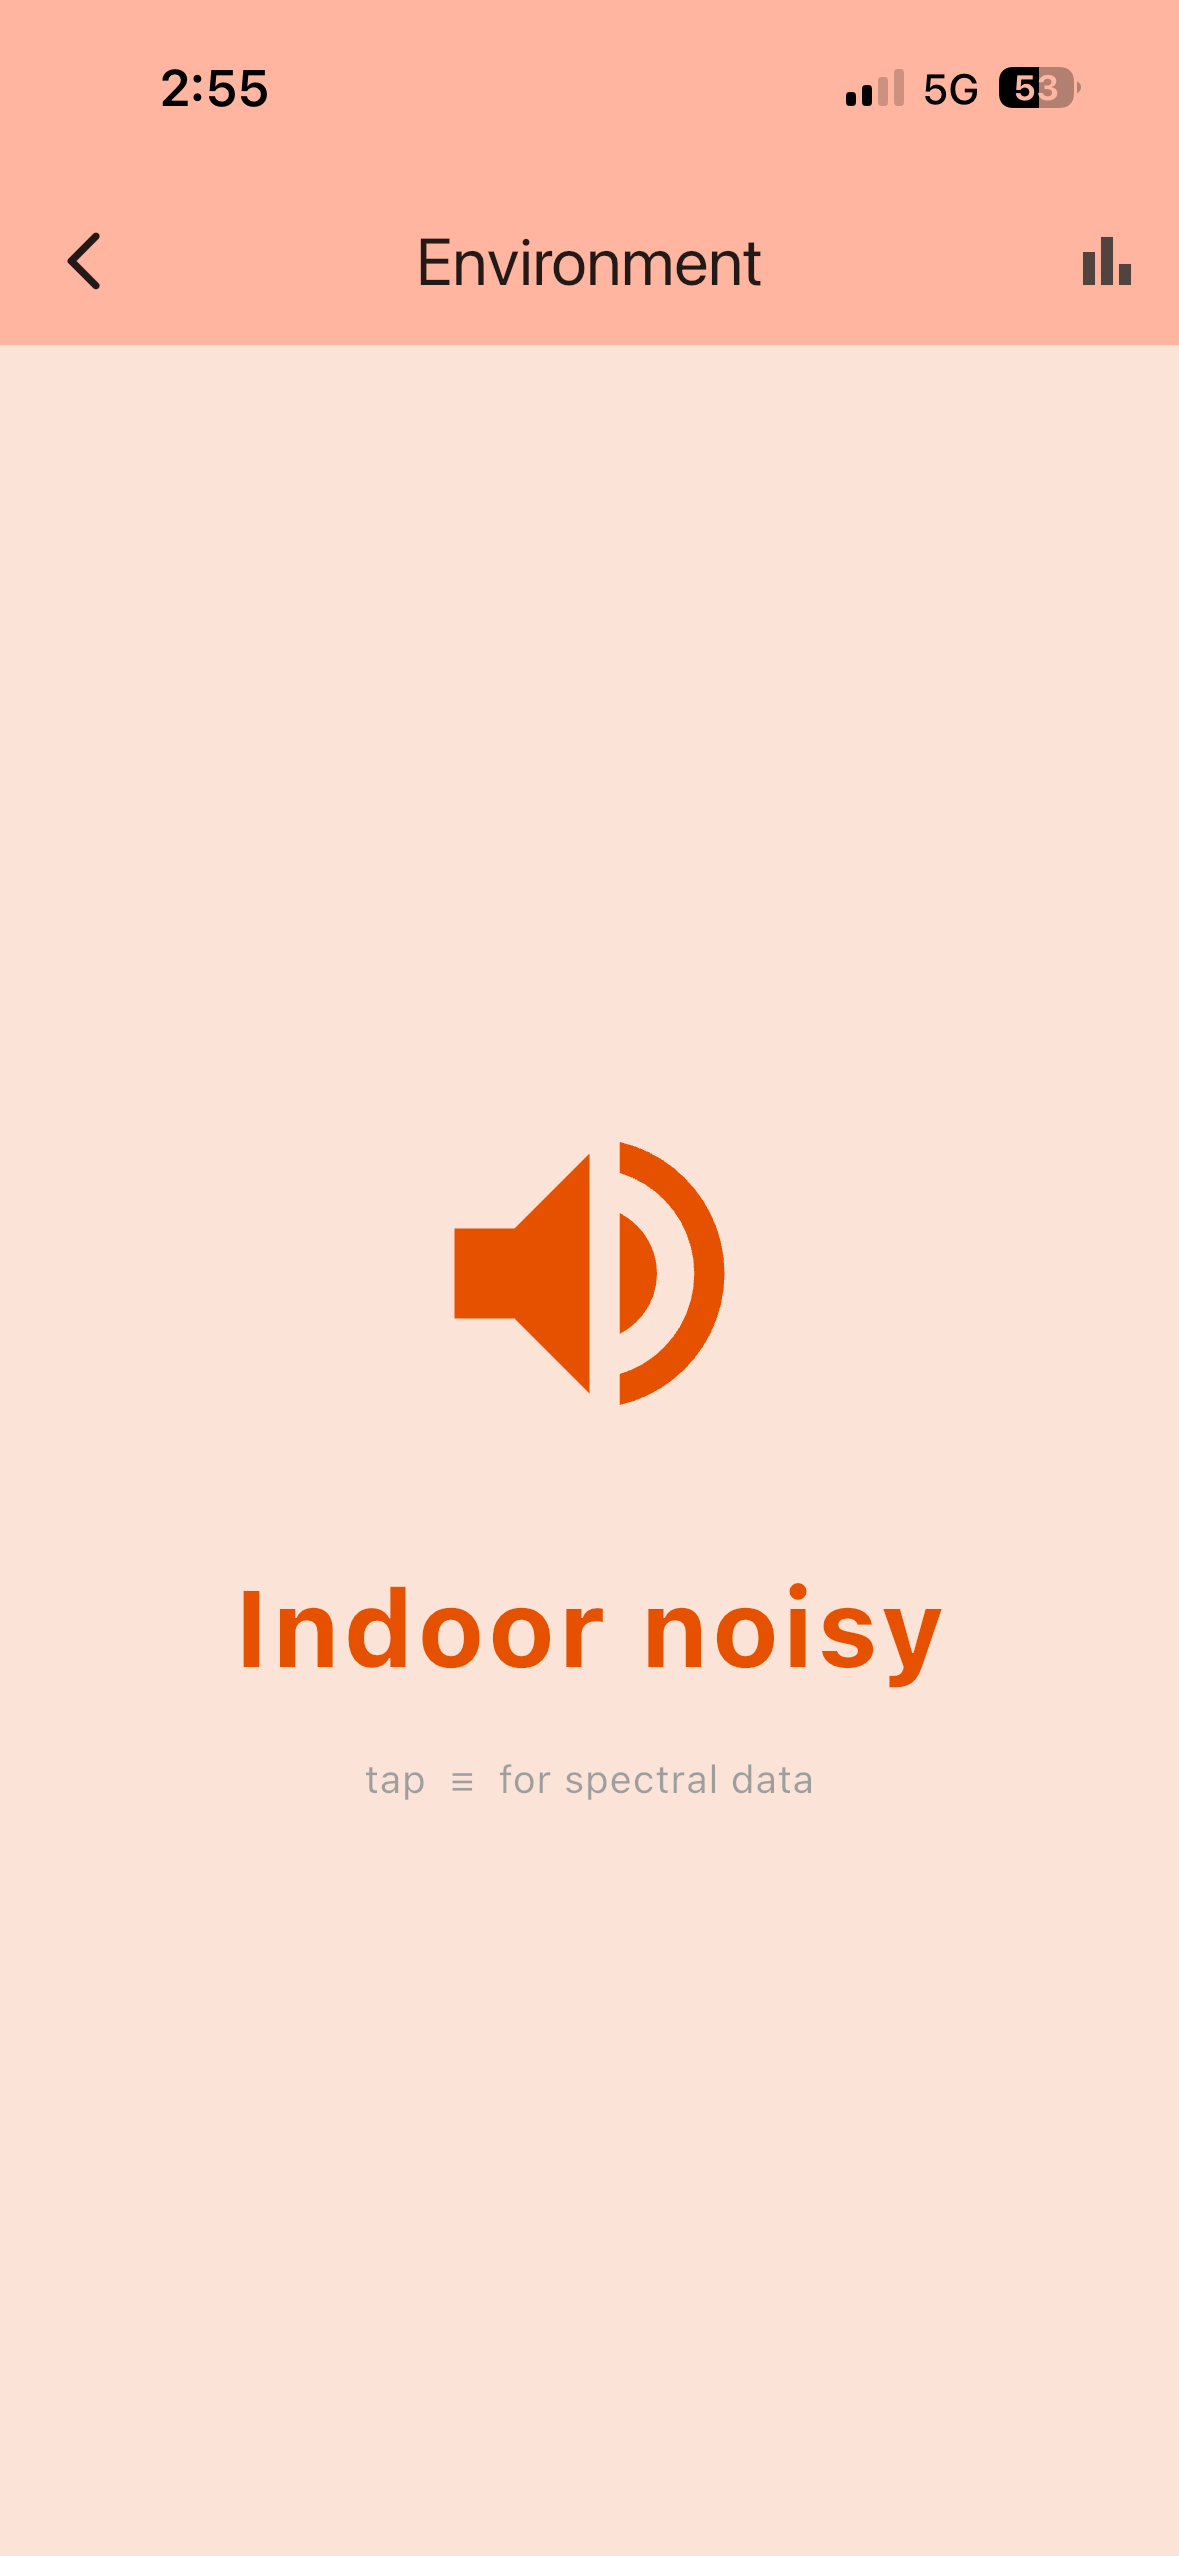
\includegraphics[width=\linewidth]{app_indoor_noisy.PNG}
        \caption{Indoor Noisy}
        \label{fig:app_indoor_noisy}
    \end{subfigure}
    \hfill
    \begin{subfigure}[t]{0.25\linewidth}
        \centering
        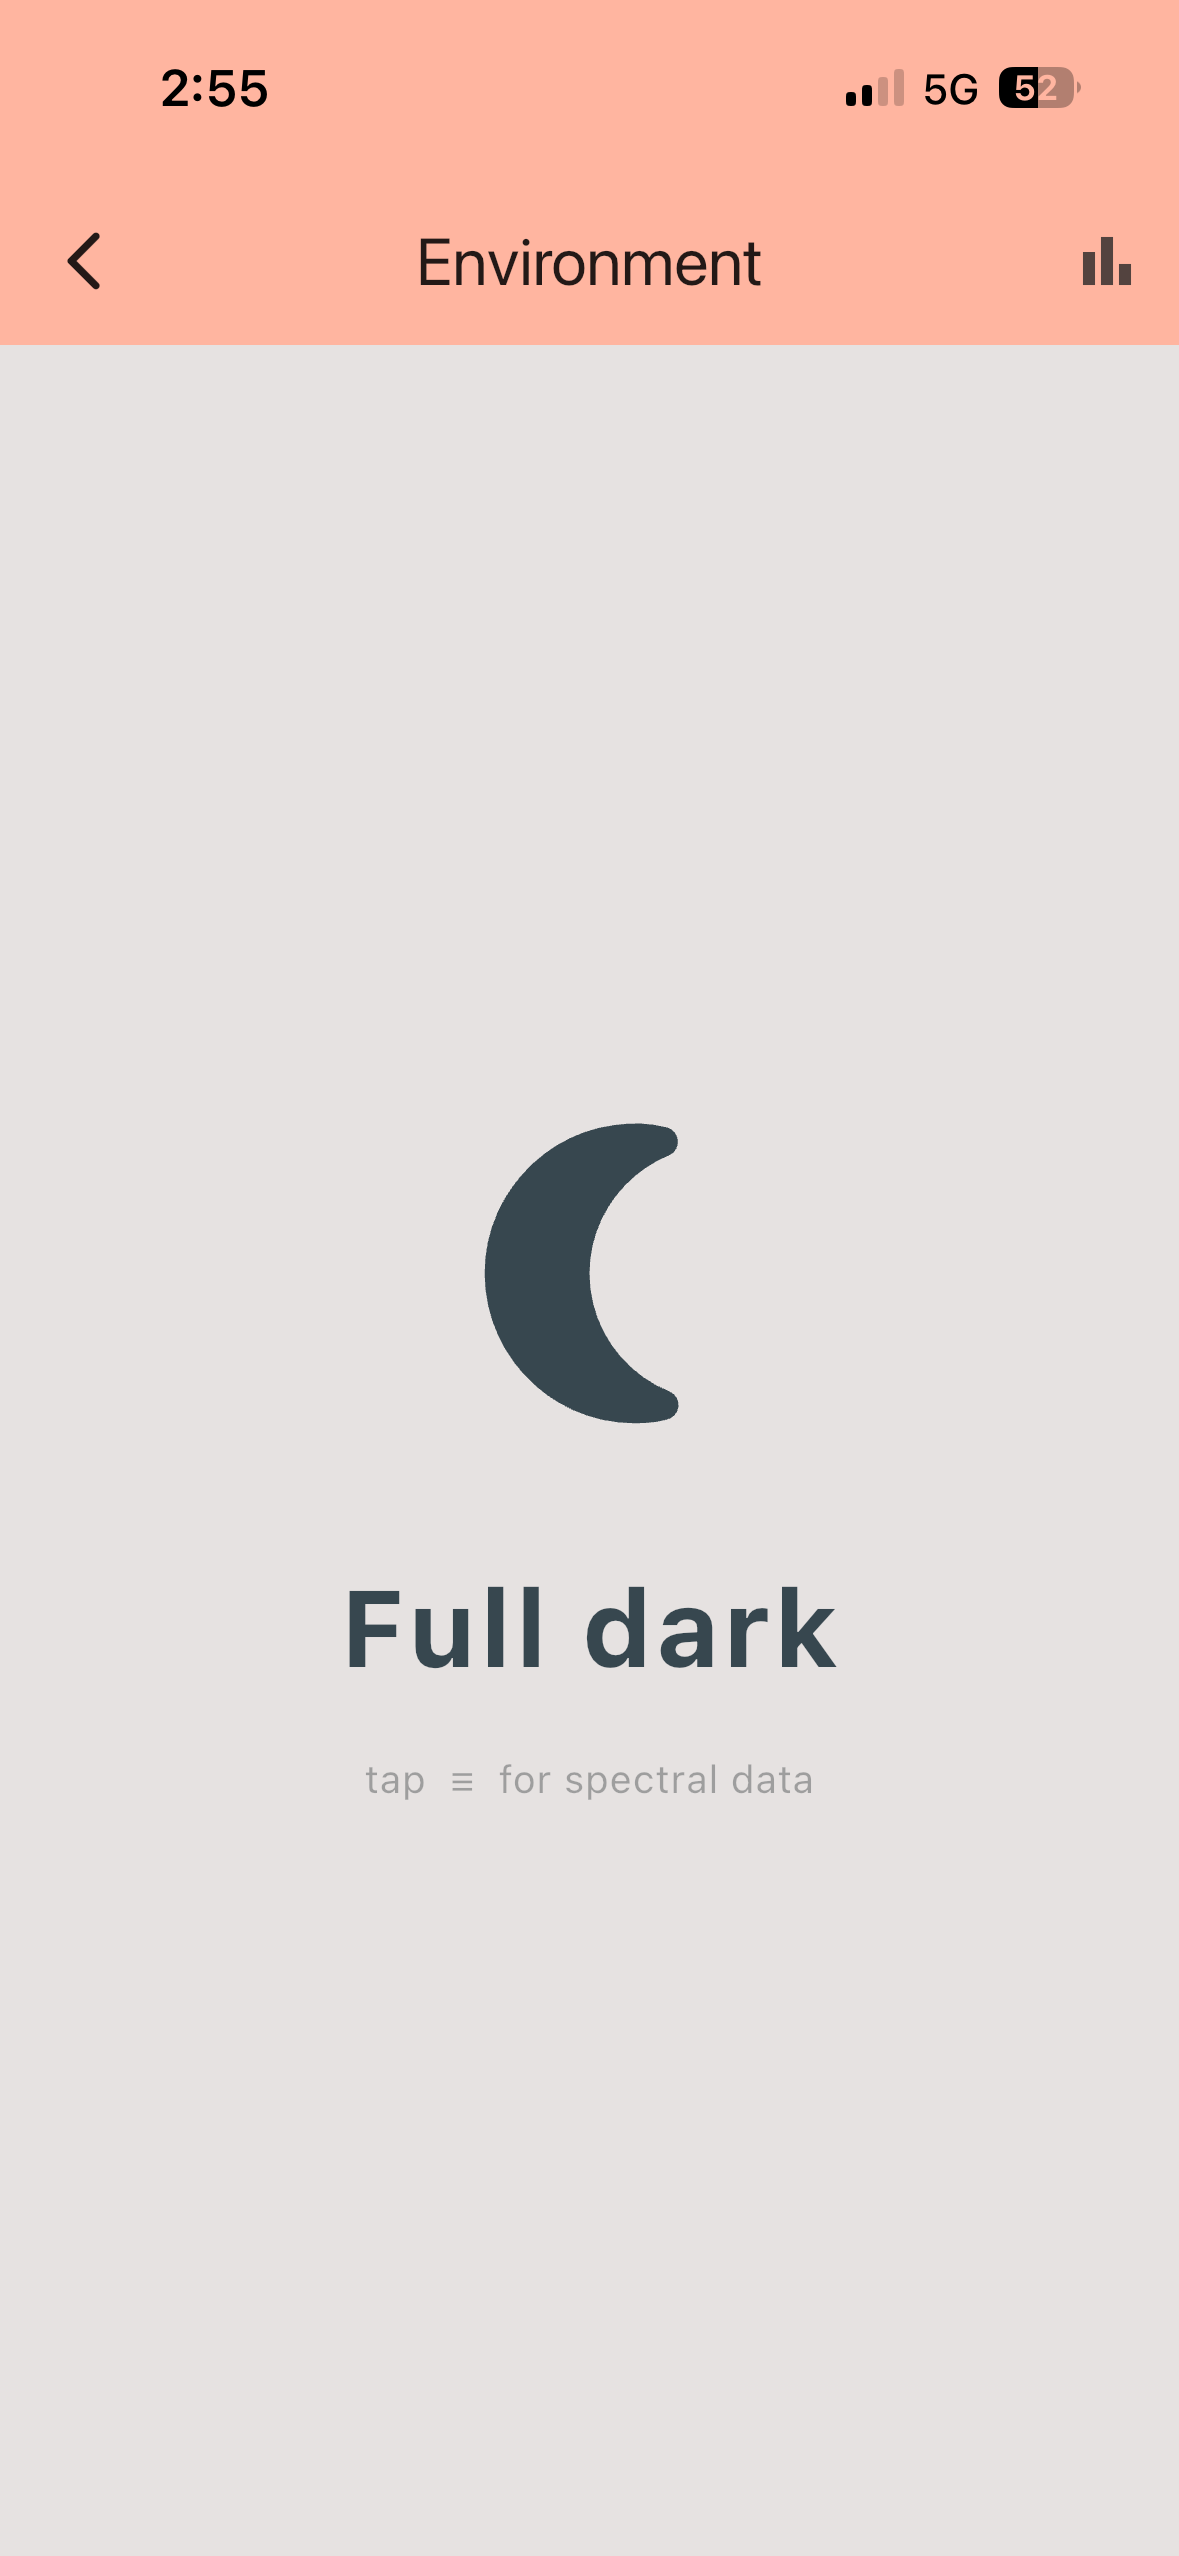
\includegraphics[width=\linewidth]{app_full_dark.PNG}
        \caption{Full Dark}
        \label{fig:app_full_dark}
    \end{subfigure}
    \hfill
    \begin{subfigure}[t]{0.25\linewidth}
        \centering
        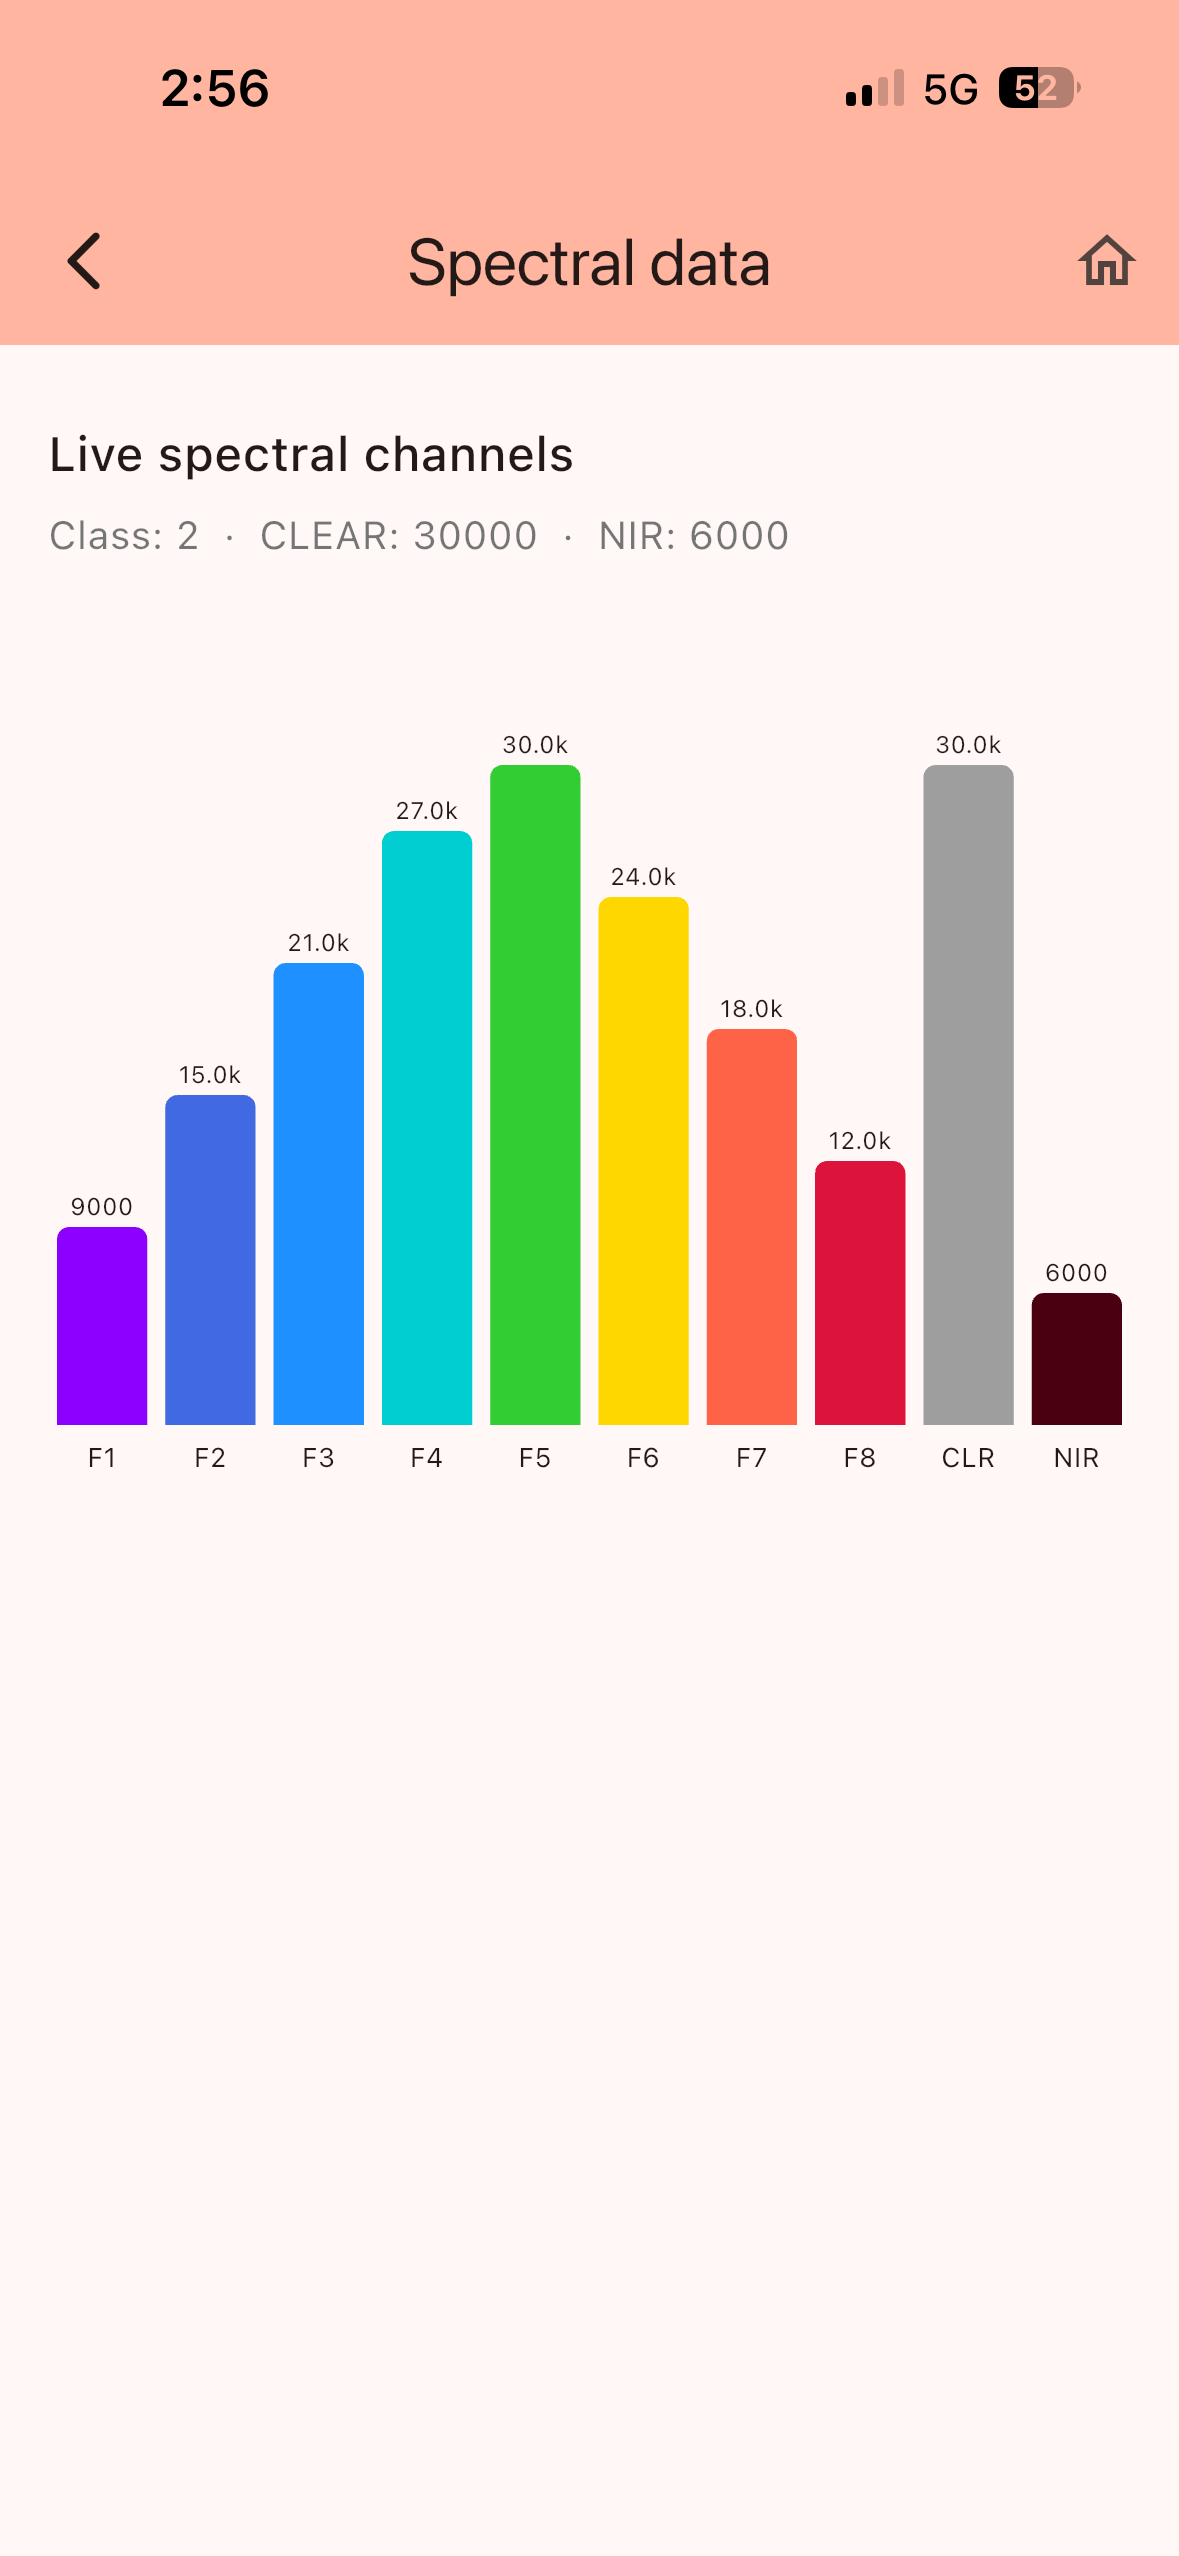
\includegraphics[width=\linewidth]{app_spectral_channels.PNG}
        \caption{Spectral Telemetry}
        \label{fig:app_spectral}
    \end{subfigure}
    \caption{Companion mobile application UI states. Classified environmental contexts received over BLE: (a) Underground, (b) Outdoor, (c) Indoor Silent (silent UI toggle), (d) Indoor Noisy, (e) Full Dark (covered). (f) Real-time raw spectrometer telemetry visualizer.}
    \label{fig:mobile_app_screens}
\end{figure}

% =========================================================================
% SECTION 6: FINAL RESULTS AND DISCUSSION (Max 250 words + Figures/Graphs)
% =========================================================================
\section{Final results and discussion}
\noindent\textbf{Contributors:} Mirko Pica (20\%), Elena Dalle Nogare (20\%), Christian Prendin (20\%), Leonardo Grossi (20\%), Jaime Iriarte (20\%)
\vspace{0.1cm}

The final integrated prototype demonstrates real-time edge context classification using fused multimodal data streams. The 8-bit quantized ANN achieves an accurcy of 0.9894 on the test set, with perfect recall in \texttt{Covered/Dark} and \texttt{Outdoor} contexts (Figure~\ref{fig:tinyml_confusion}). Localized acoustic similarities between the \texttt{Indoor Quiet} and \texttt{Indoor Normal} classes form the primary classification bottleneck. Due to the small validation dataset size, these accuracy figures are likely overoptimistic for unstructured real-world generalization.

\subsection{Low-Power Architecture and Power Analysis}
To satisfy wearable power constraints, the STM32U575 firmware transitions to a decoupled, thread-mode execution model. The GPDMA and EXTI interrupts handle lightweight data buffering and set atomic request flags, offloading the heavy feature extraction and model execution to the main thread. 

When idle, the CPU enters Wait-For-Interrupt (WFI) sleep mode, gating the core clock while MDF1 and GPDMA1 continue acquiring data autonomously in SRAM. A critical section via \texttt{\_\_disable\_irq()} prevents sleep-race conditions. 

At a stride of 9 blocks, active processing runs for 60~ms every 3.43~seconds (1.75\% duty cycle). As shown in Table~\ref{tab:power_consumption}, this results in an average current draw of 2.08~mA, yielding an overall 88.2\% reduction in core current compared to continuous polling.

\begin{table}[H]
\centering
\resizebox{\columnwidth}{!}{%
\begin{tabular}{lcc}
\toprule
\textbf{Operating Mode} & \textbf{Core Current (mA)} & \textbf{Duty Cycle} \\
\midrule
\textbf{Continuous Polling (Active-Run)} & 17.60 & 100.00\% \\
\midrule
\textbf{Low-Power Decoupled (WFI):} & & \\
- Active Processing (60~ms) & 17.60 & 1.75\% \\
- Gated Idle (Sleep, 3.37~s) & 1.80 & 98.25\% \\
- \textit{Weighted Average} & \textbf{2.08} & \textbf{100.00\%} \\
\midrule
\textbf{Overall Current Reduction} & \multicolumn{2}{c}{\textbf{88.2\% savings}} \\
\bottomrule
\end{tabular}%
}
\caption{Power consumption comparison between continuous polling and the decoupled low-power firmware on the STM32U575 core.}
\label{tab:power_consumption}
\end{table}

\subsection{Short Video Demonstration}
A video showcasing the product presentation and a real-world demonstration of the system is available at: \\
\href{run:LUMIA.mp4}{LUMIA.mp4}

\begin{figure}[H]
    \centering
    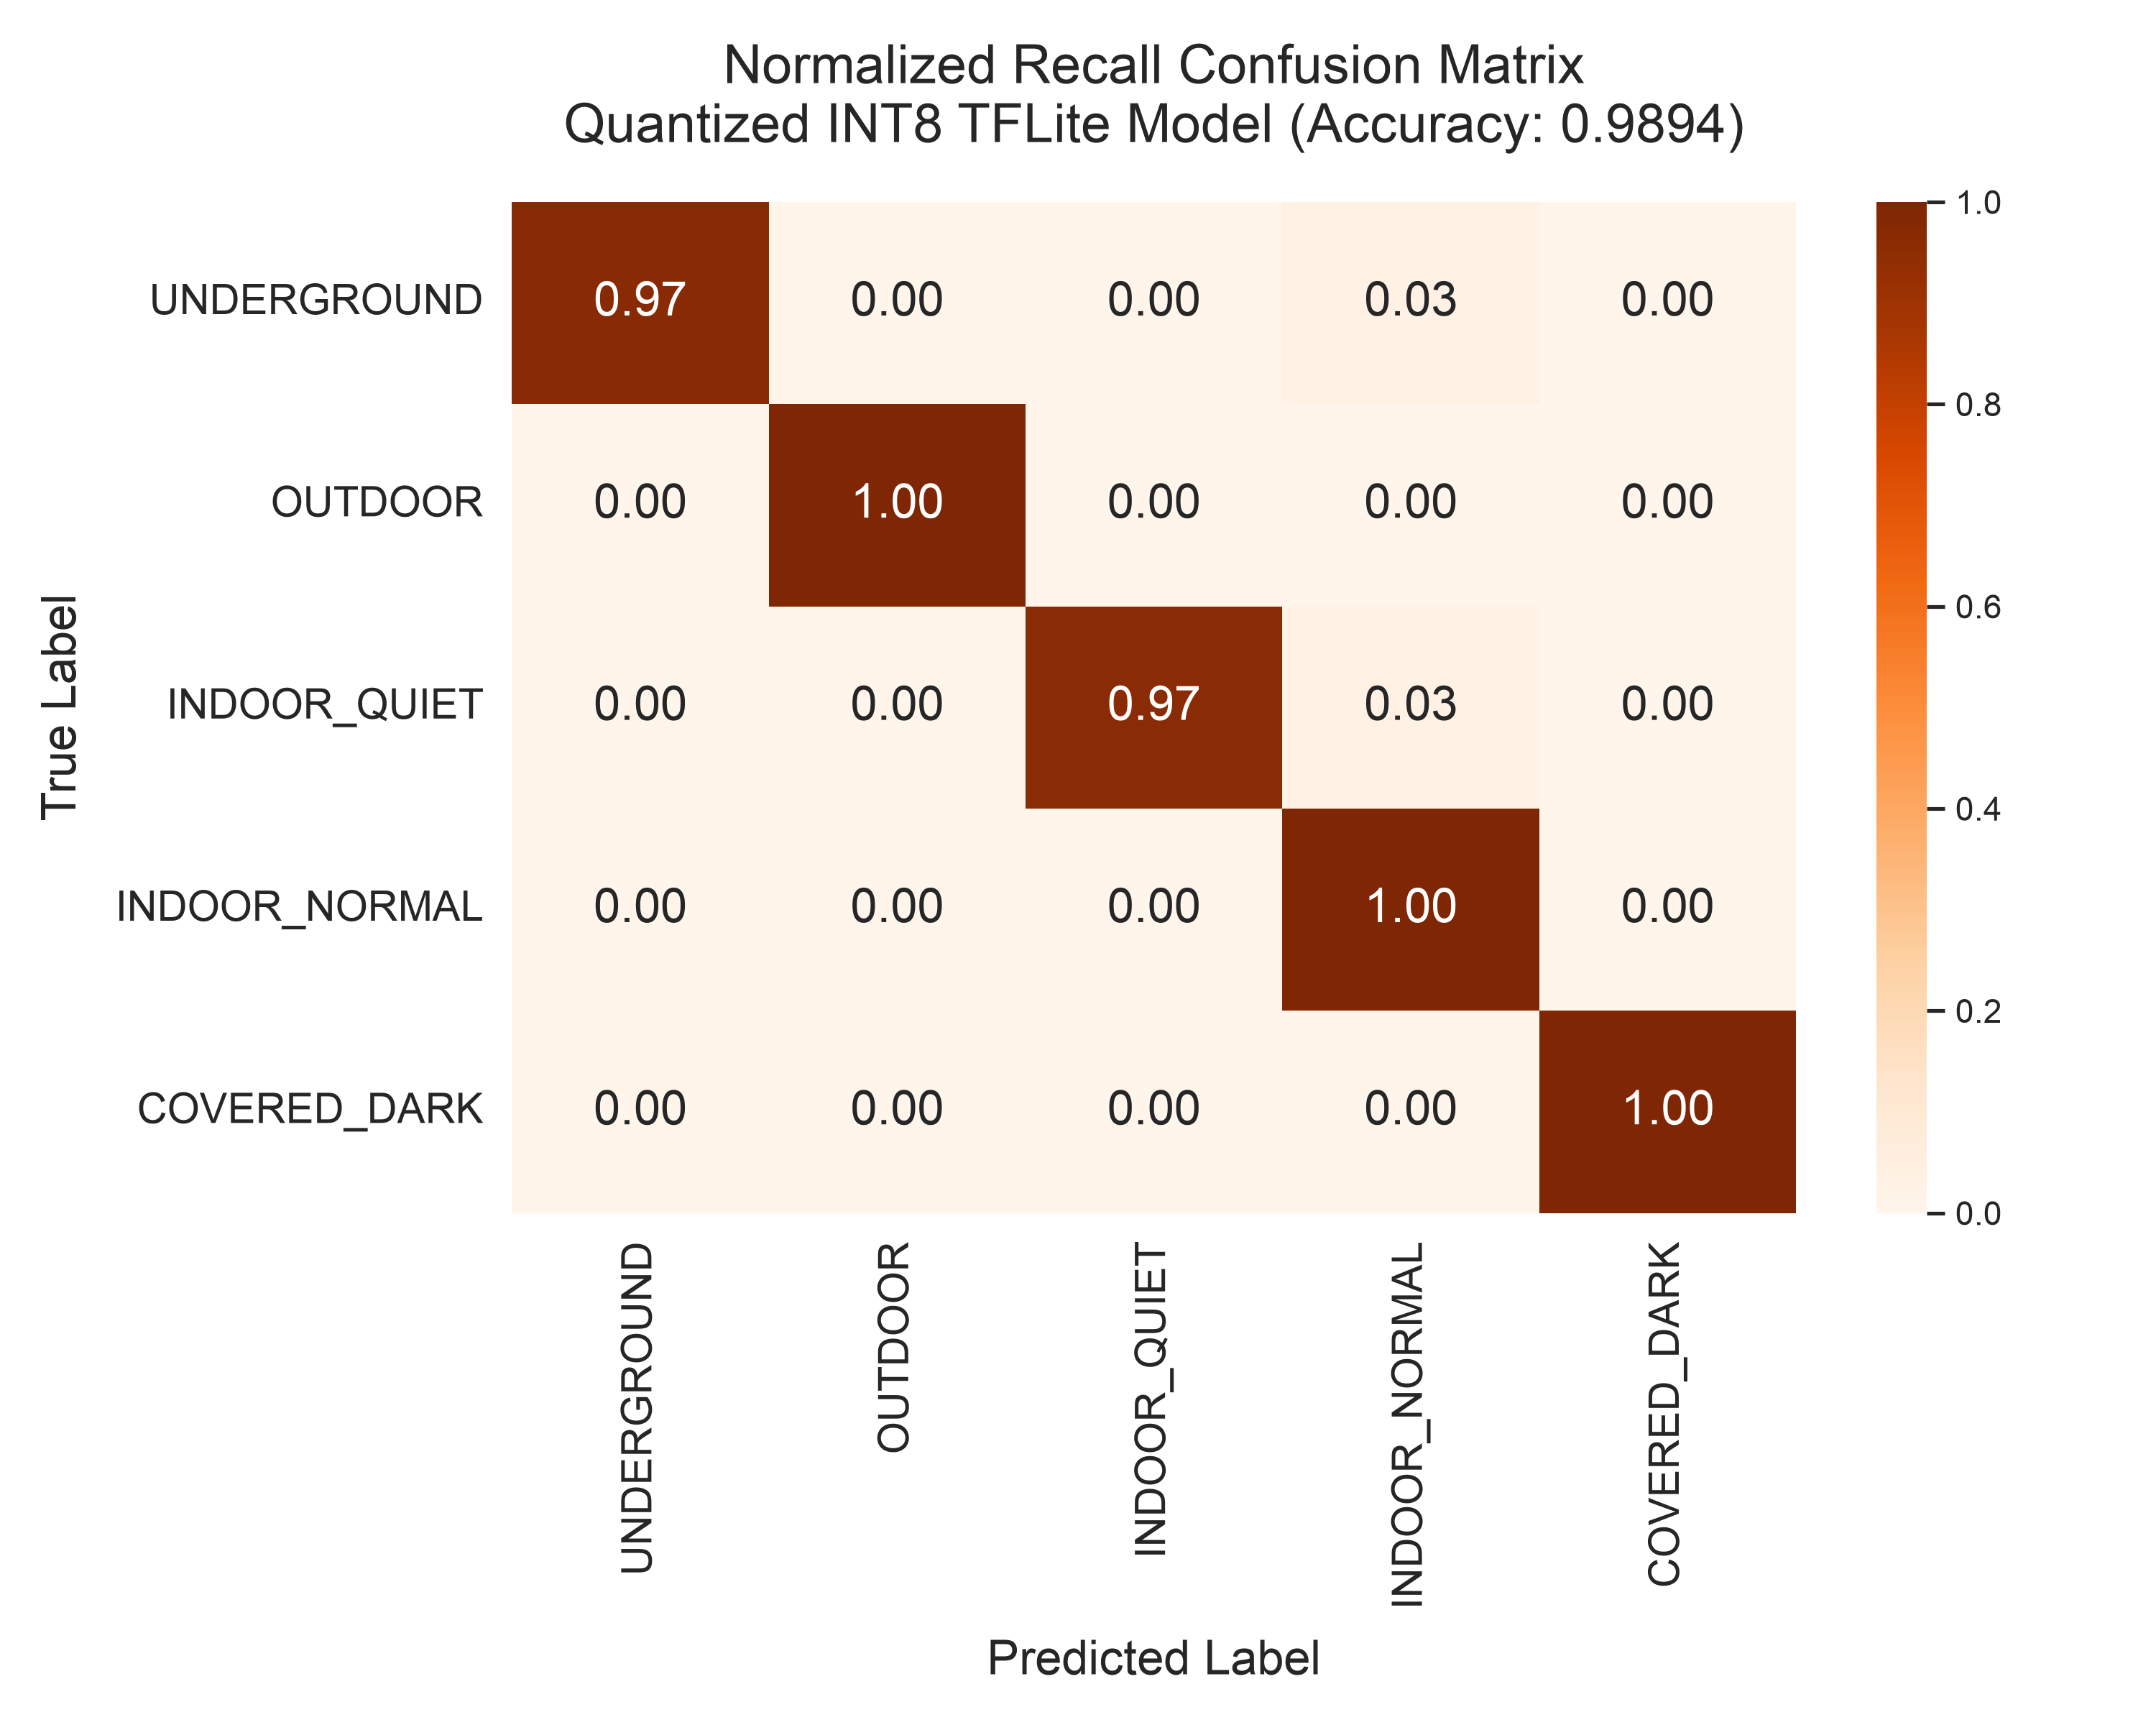
\includegraphics[width=0.85\linewidth]{tinyml_confusion_matrix.png}
    \caption{Normalized recall confusion matrix for the on-chip 8-bit quantized TinyML neural network executing local 5-class context inference.}
    \label{fig:tinyml_confusion}
\end{figure}

\end{multicols}

\newpage
% =========================================================================
% SECTION 7 & 8: ATTACHMENTS & FIGURES
% =========================================================================
\section*{Attachments}

% Figure 1: Probe Assembly
\begin{figure}[H]
    \centering
    \begin{subfigure}[t]{0.45\textwidth}
        \centering
        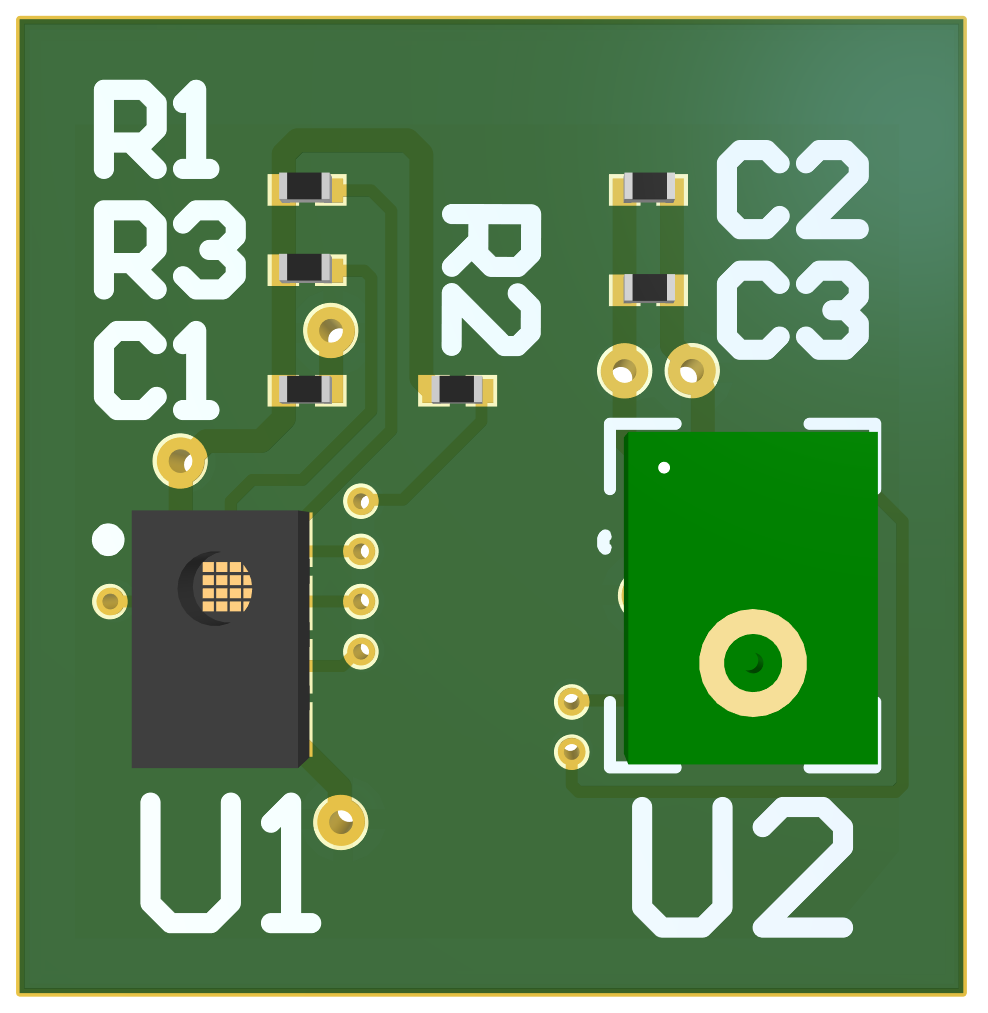
\includegraphics[width=\linewidth]{Top side PCB.png}
        \caption{}
        \label{fig:lumos_top}
    \end{subfigure}
    \hfill
    \begin{subfigure}[t]{0.45\textwidth}
        \centering
        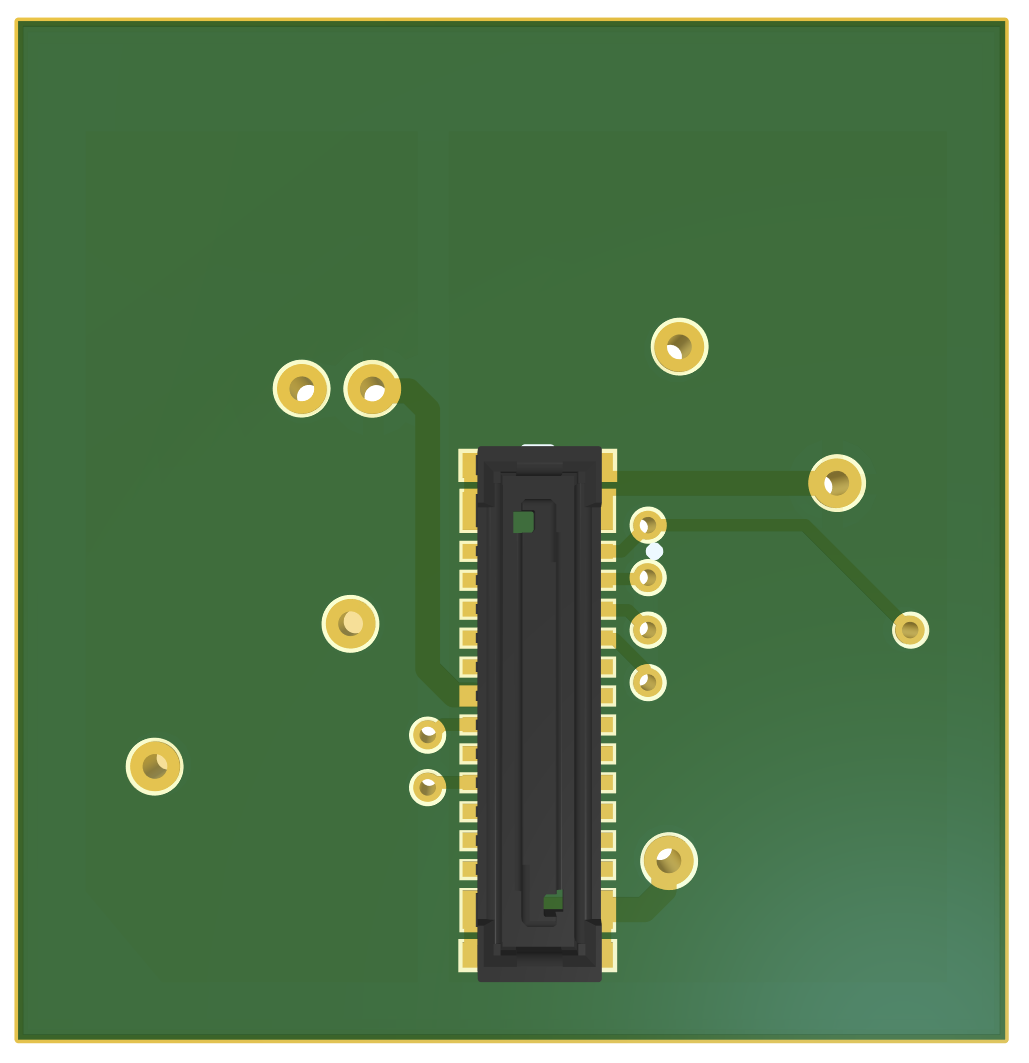
\includegraphics[width=\linewidth]{Bottom side PCB.png}
        \caption{}
        \label{fig:lumos_bottom}
    \end{subfigure}
    \caption{(a) Top side of the custom LUMOS sensor probe PCB, including the AS7341 multispectral light sensor and the IMP34DT05TR digital MEMS microphone. (b) Bottom side of the custom LUMOS sensor probe PCB, showing the board-to-board connector used to interface the probe with the smart-glasses platform.}
    \label{fig:lumos_probe}
\end{figure}

% Figure 2: Electrical Schematics Grid
\begin{figure}[H]
    \centering
    \begin{minipage}[c]{0.48\textwidth}
        \centering
        \begin{subfigure}{\linewidth}
            \centering
            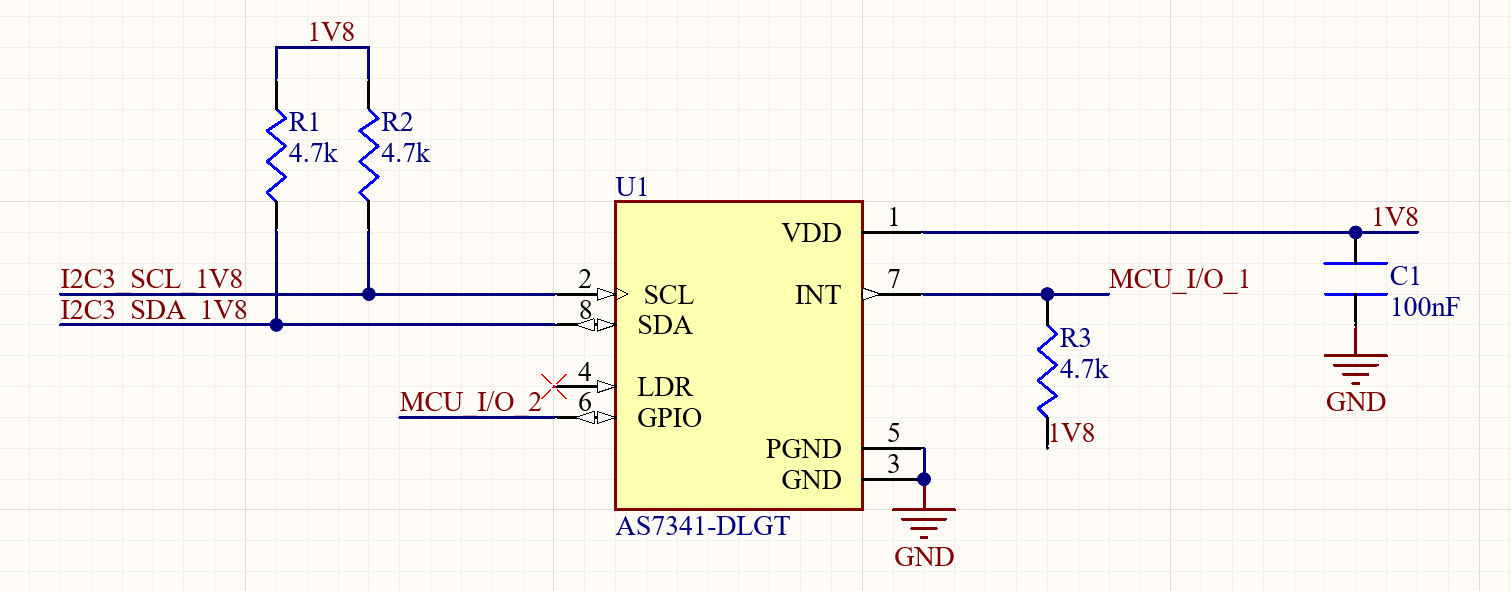
\includegraphics[width=\linewidth]{Light Sensor AS7341.png}
            \caption{}
            \label{fig:light_sensor_schematic}
        \end{subfigure}
        \vspace{0.4cm}
        \begin{subfigure}{\linewidth}
            \centering
            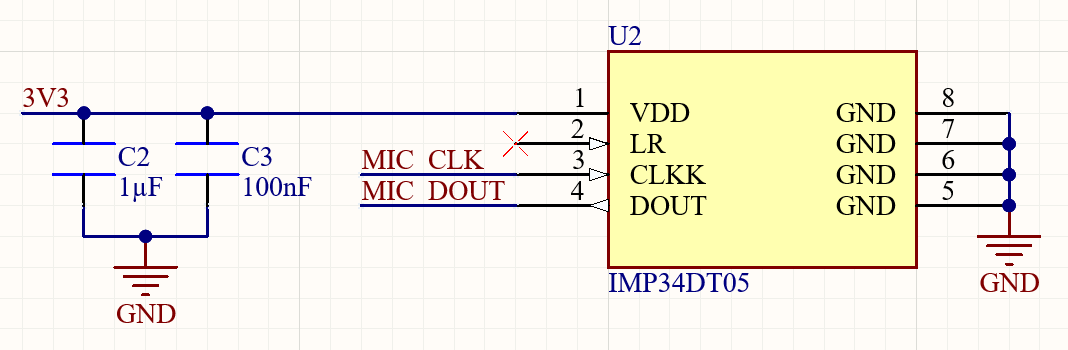
\includegraphics[width=\linewidth]{Microphone IMP34DT05.png}
            \caption{}
            \label{fig:microphone_schematic}
        \end{subfigure}
    \end{minipage}
    \hfill
    \begin{minipage}[c]{0.48\textwidth}
        \centering
        \begin{subfigure}{\linewidth}
            \centering
            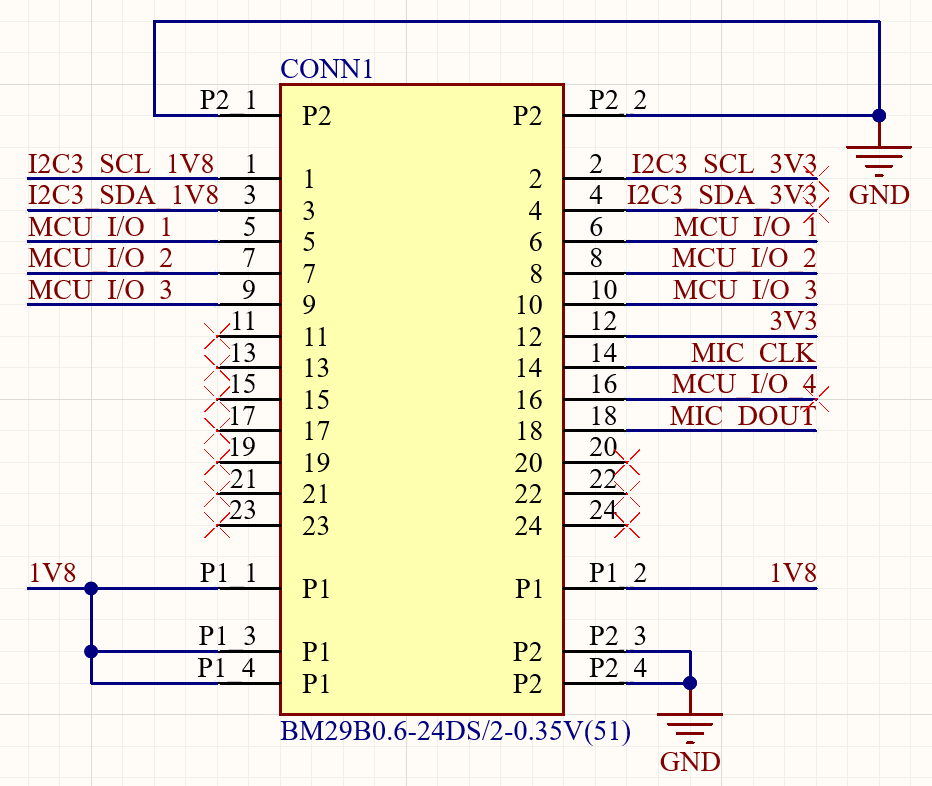
\includegraphics[height=7.1cm, keepaspectratio]{CONN Scheme.png}
            \caption{}
            \label{fig:connector_schematic}
        \end{subfigure}
    \end{minipage}
    \caption{(a) Schematic of the AS7341 multispectral sensor interface. (b) Schematic of the IMP34DT05TR digital MEMS microphone interface. (c) Board-to-board connector schematic used to interface the LUMOS probe with the main board.}
    \label{fig:lumos_schematics}
\end{figure}

% Figure 3: Data Logger and Inference Pipelines
\begin{figure}[H]
    \centering
    \begin{subfigure}[b]{0.8\textwidth}
        \centering
        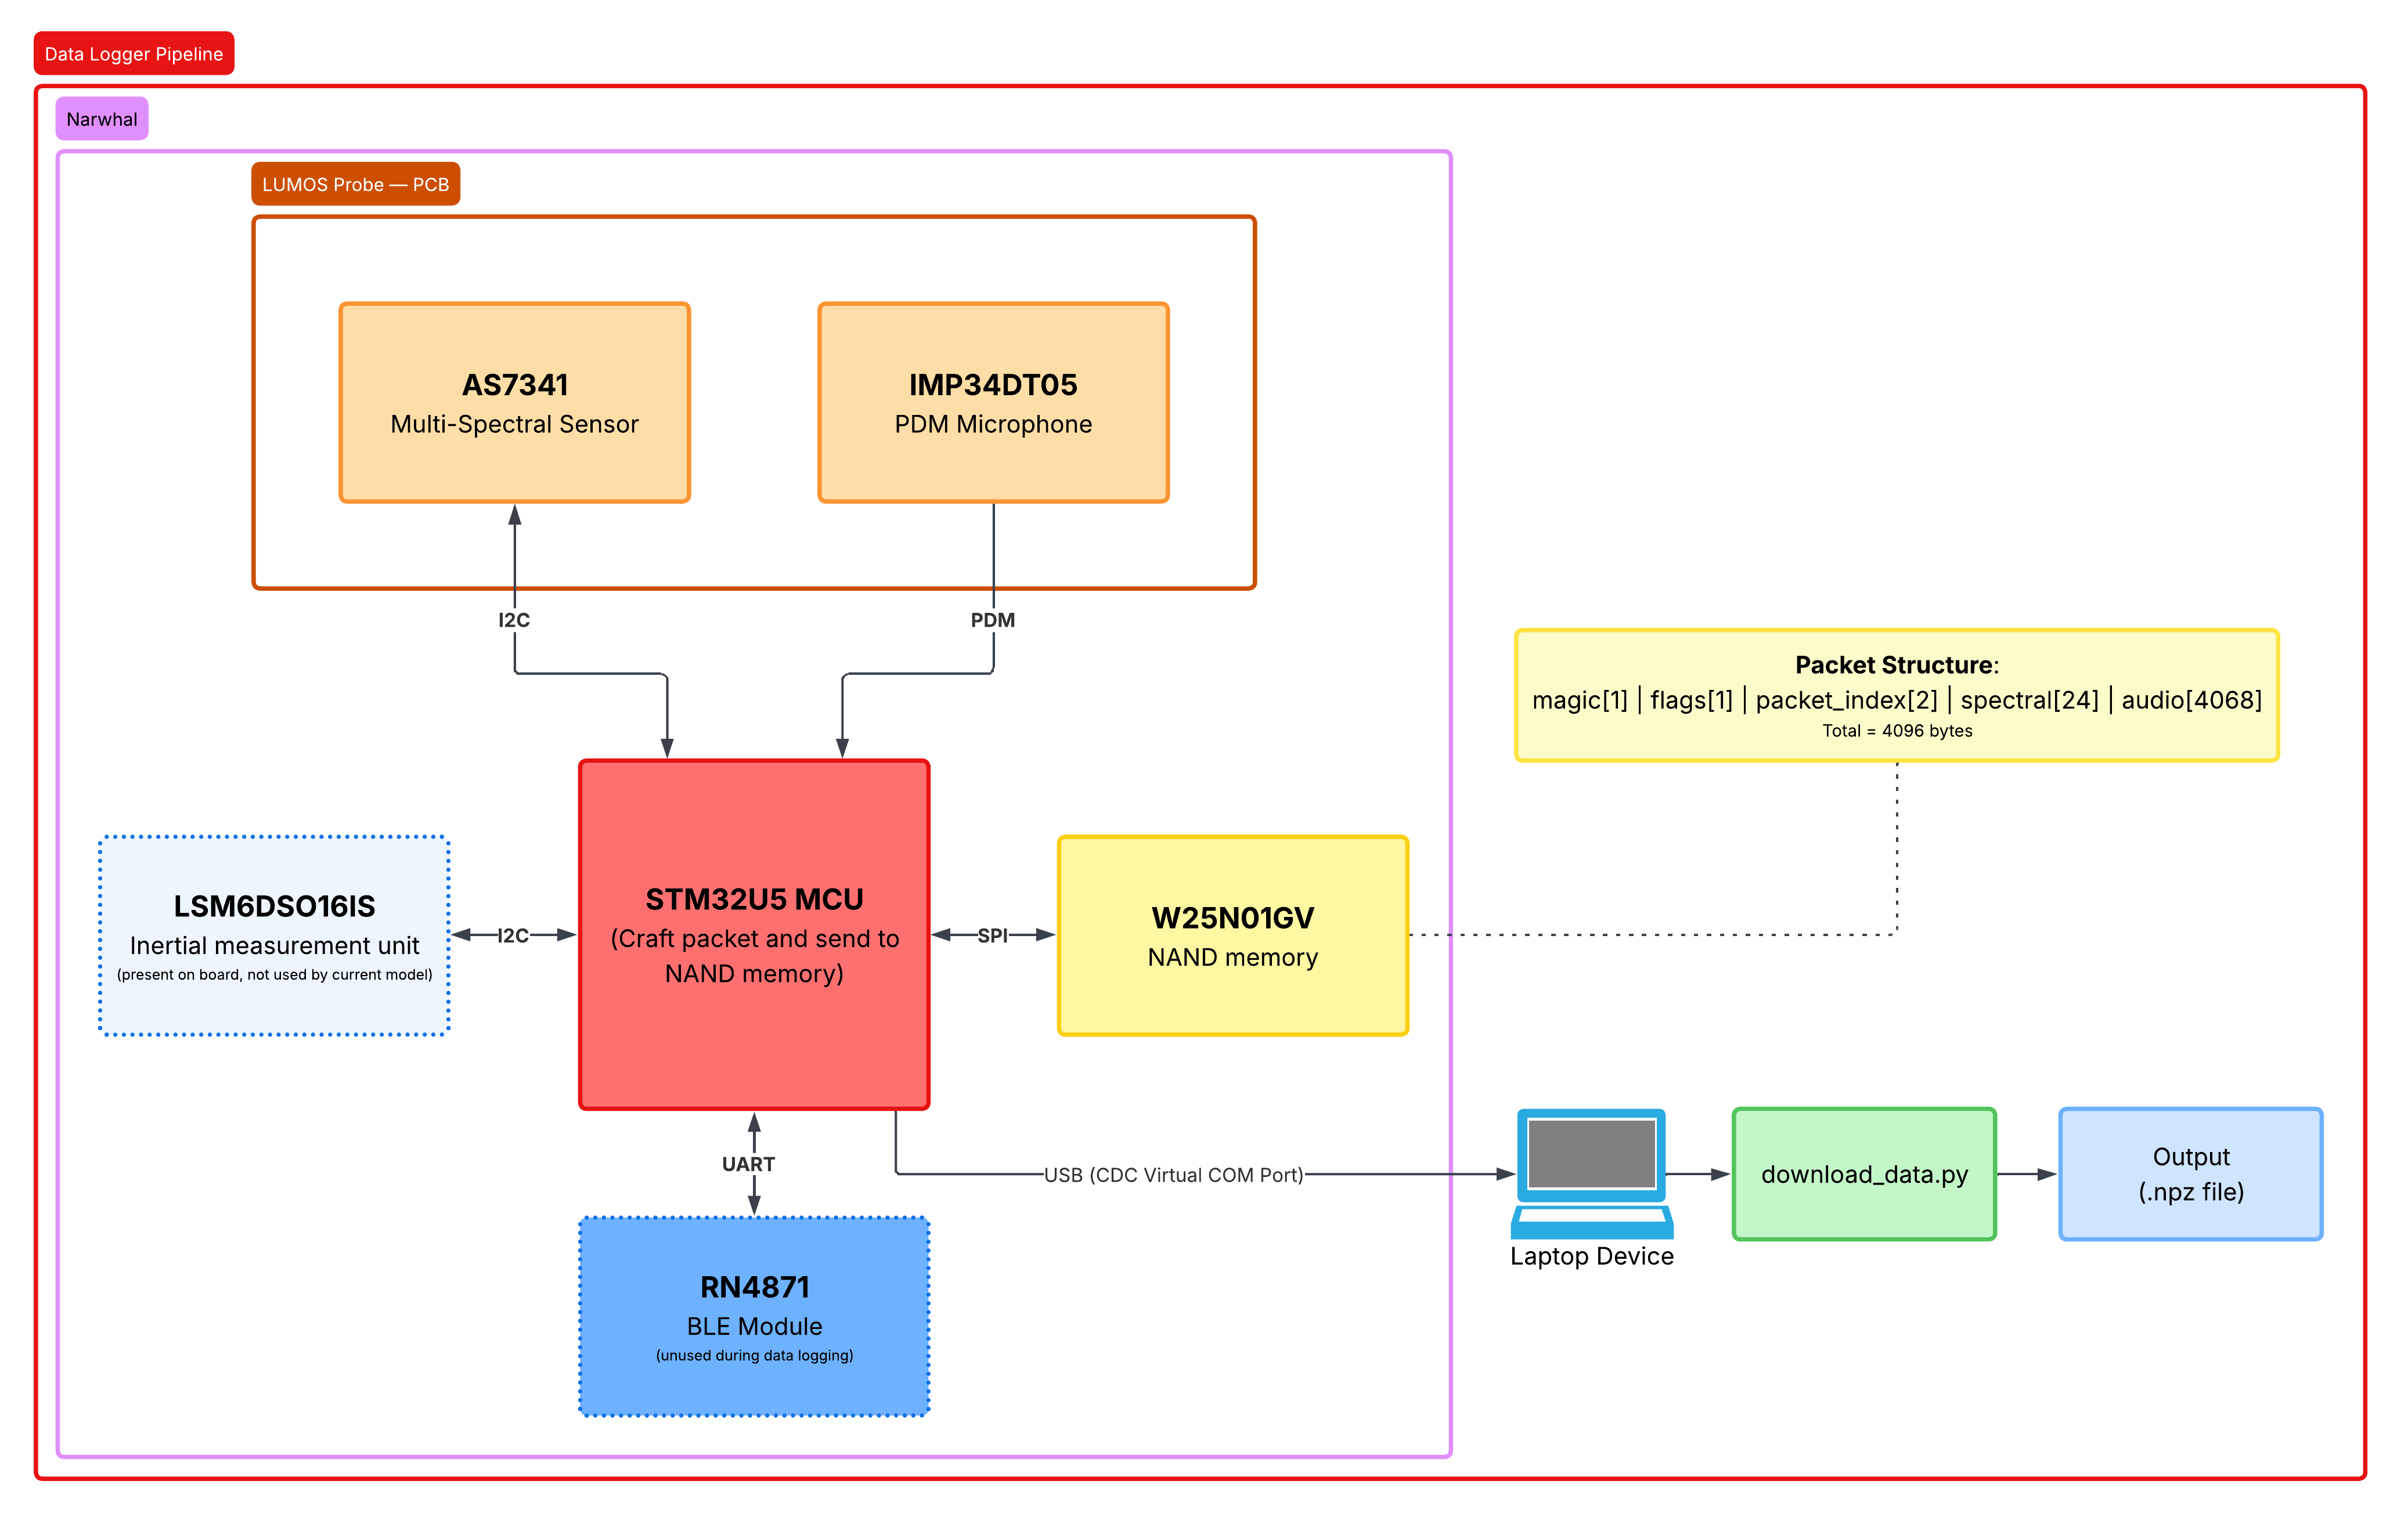
\includegraphics[width=\linewidth]{data_logger_pipeline_scheme.png}
        \caption{}
        \label{fig:data_logger_pipeline}
    \end{subfigure}
    \\
    \vspace{0.4cm}
    \begin{subfigure}[b]{0.8\textwidth}
        \centering
        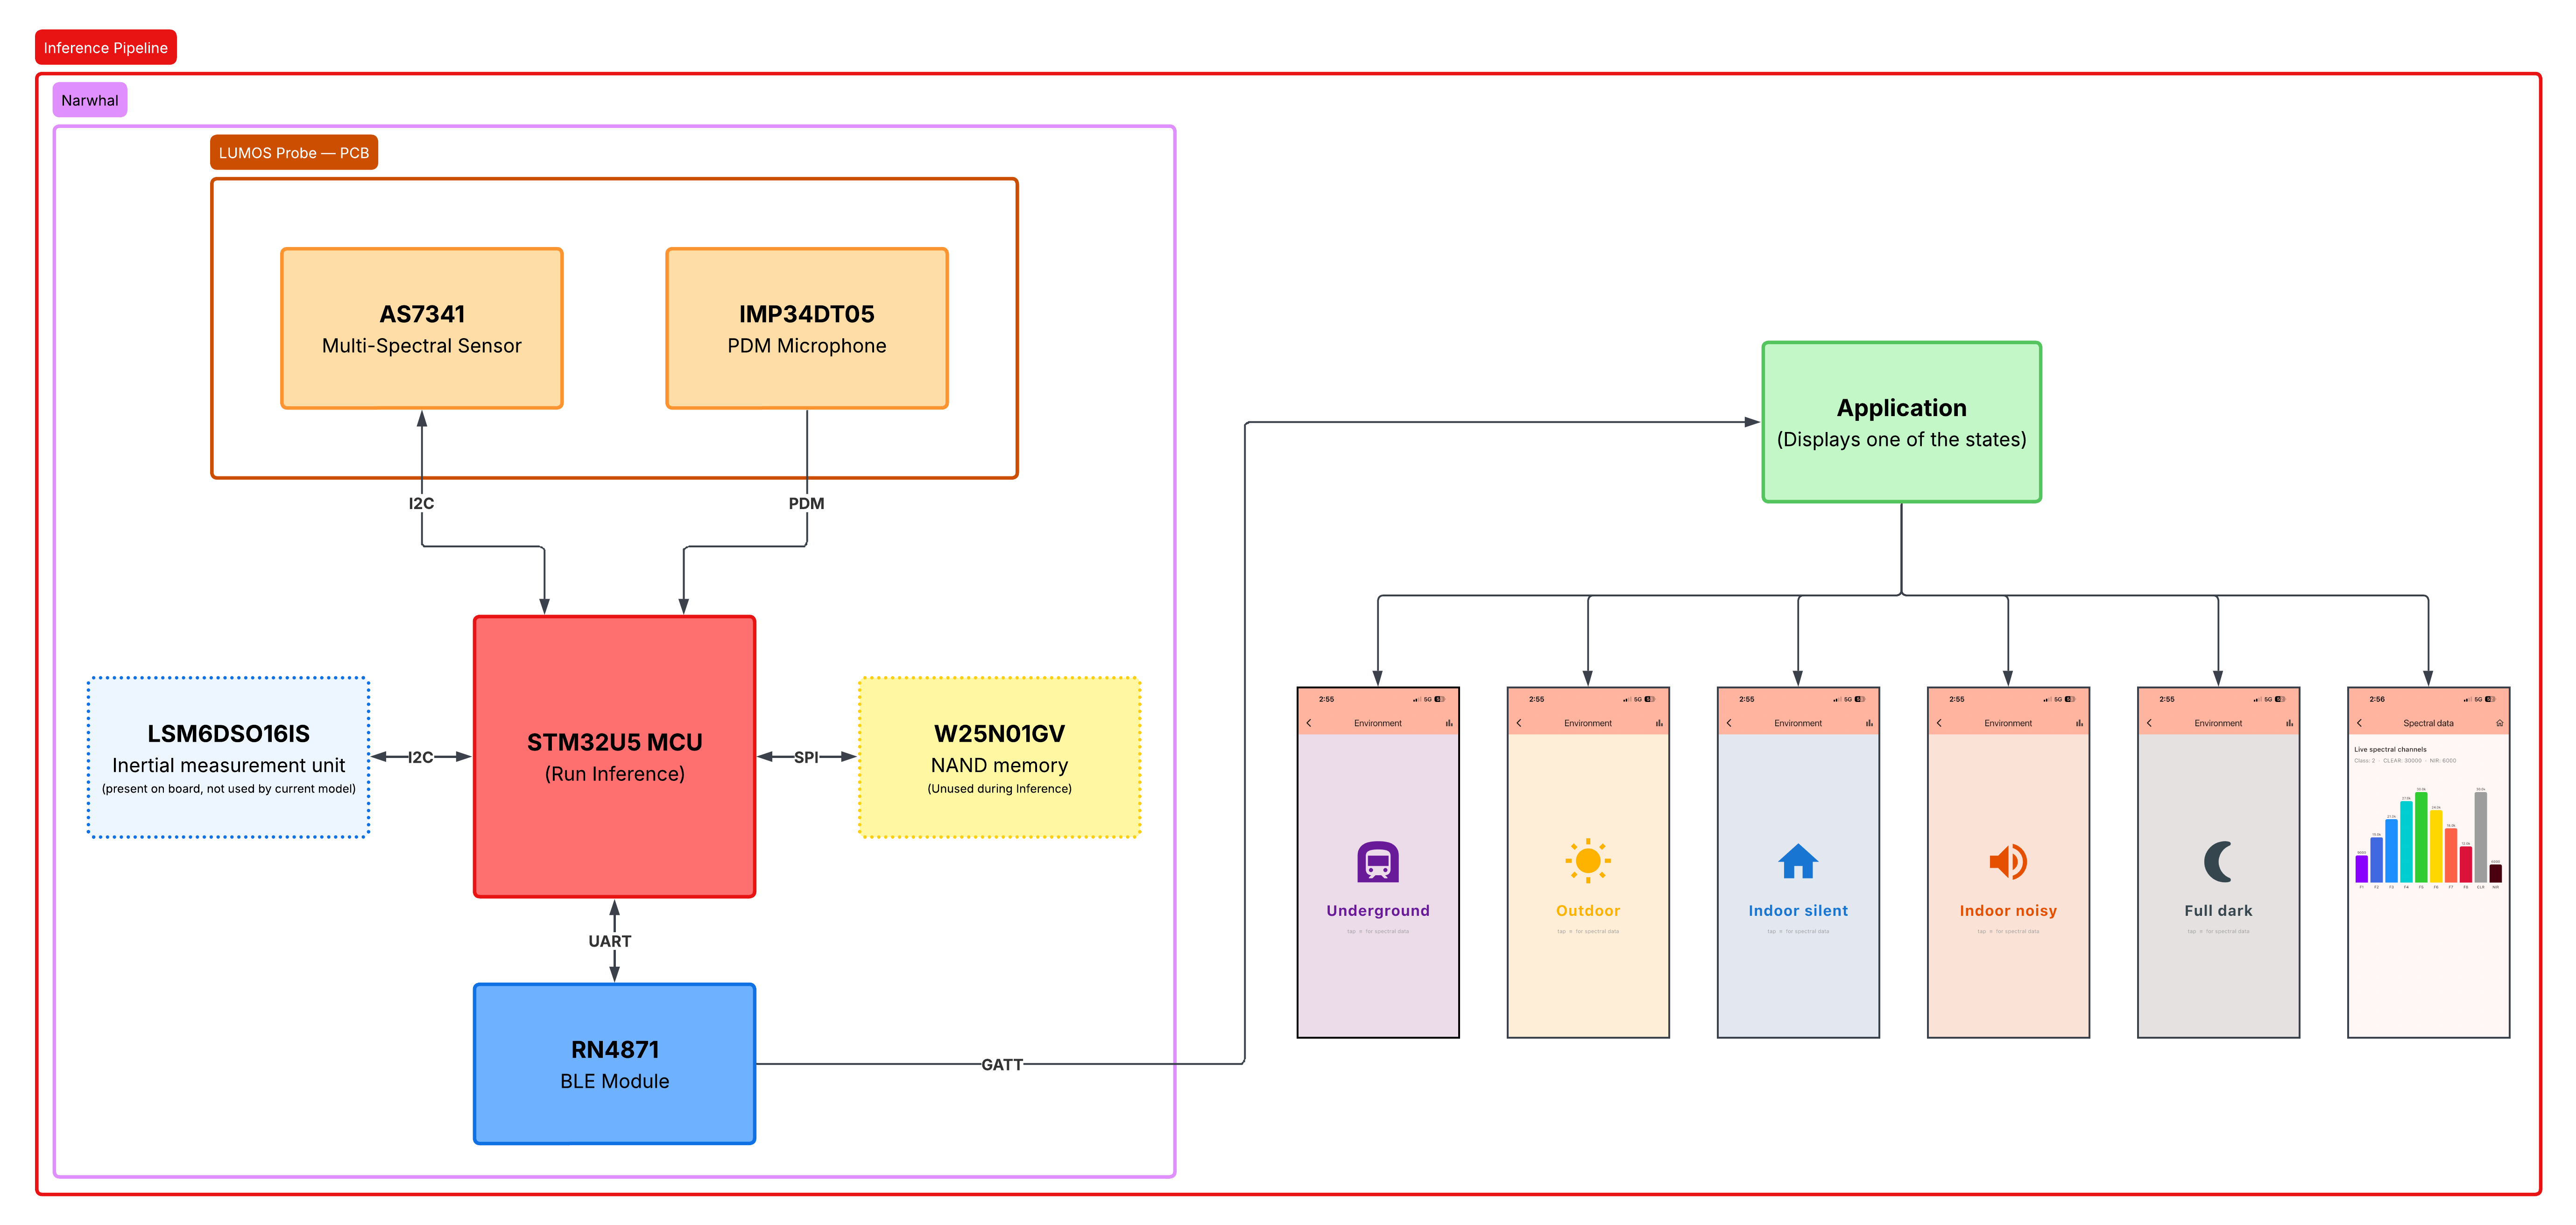
\includegraphics[width=\linewidth]{inference_pipeline_scheme.png}
        \caption{}
        \label{fig:inference_pipeline}
    \end{subfigure}
    \caption{Functional system pipeline architectures: (a) Data logger acquisition and NAND flash streaming pipeline. (b) Edge TinyML inference pipeline utilizing GPDMA double buffering, asynchronous thread-mode feature calculation, and atomic WFI low-power sleep transitions.}
    \label{fig:pipeline_schemes}
\end{figure}

% Figure 4: Neural Network Training Scheme
\begin{figure}[H]
    \centering
    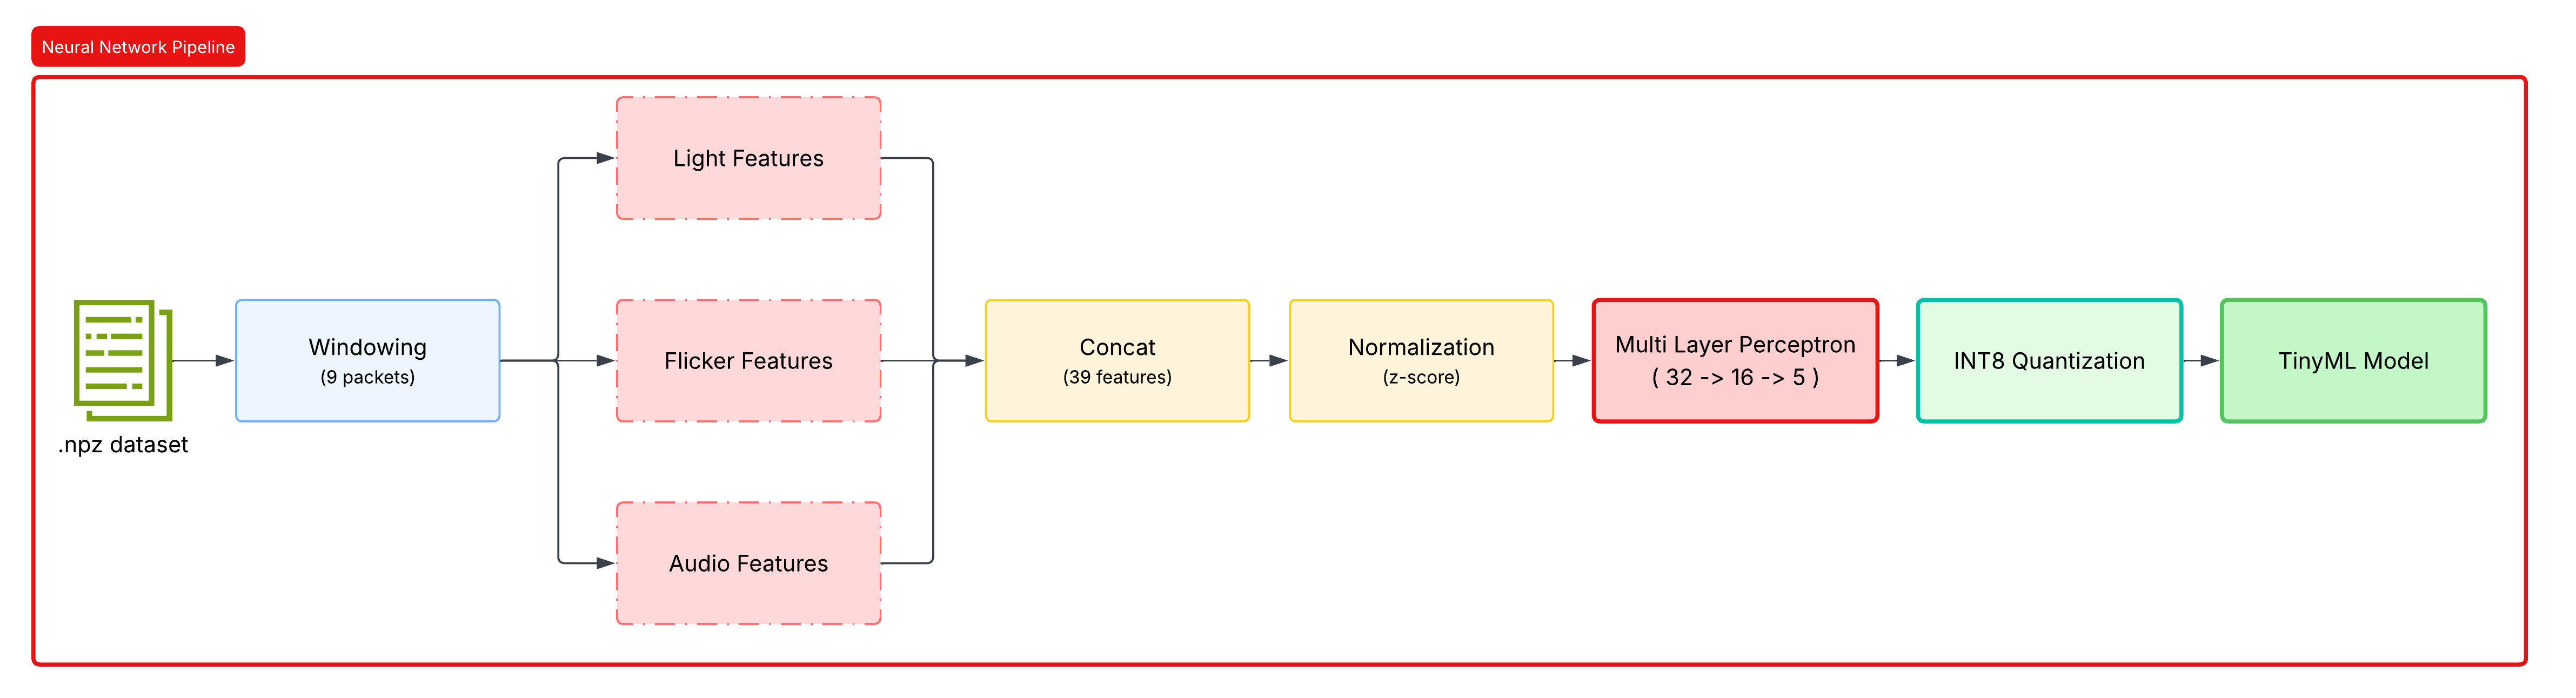
\includegraphics[width=0.8\textwidth]{nn_pipeline_scheme.png}
    \caption{Neural network feature collection, feature normalization, and classification pipeline.}
    \label{fig:nn_pipeline_scheme}
\end{figure}

\end{document}